% GENERATED by scripts/build_latex.py -- do not edit by hand.
% The Markdown chapters in dissertation/ are the source of truth; rebuild
% with `python scripts/build_latex.py` after editing them.
\documentclass[12pt]{report}
\usepackage[a4paper, margin=1in]{geometry}
\usepackage{graphicx}
\usepackage{setspace}
\usepackage{fancyhdr}
\usepackage{titlesec}
\usepackage{caption}
\usepackage{longtable}
\usepackage{tocloft}
\usepackage{enumitem}
\usepackage{amsmath}
\usepackage[hidelinks]{hyperref}

\setlength{\parindent}{0pt}
\setlength{\parskip}{0.8em}
\onehalfspacing
\sloppy

% The template's contents page lists chapters as "CHAPTER 1: INTRODUCTION",
% so the chapter heading is formatted to match rather than the report
% class's default "Chapter 1 / Title" on two lines.
\titleformat{\chapter}[hang]
  {\normalfont\Large\bfseries\MakeUppercase}{\chaptertitlename\ \thechapter:}{0.5em}{}
\titlespacing*{\chapter}{0pt}{0pt}{20pt}

\pagestyle{fancy}
\fancyhf{}
\rhead{\small A Fully-Automatic Spatial-Relationship Annotation Pipeline}
\cfoot{\thepage}
\renewcommand{\headrulewidth}{0.4pt}

\begin{document}

%==================== Title page ====================
\begin{titlepage}
\begin{center}
    \vspace*{1cm}
    {\LARGE \textbf{A Fully-Automatic Spatial-Relationship\\[0.3cm]
     Annotation Pipeline for Robot-Acquired Images,\\[0.3cm]
     Validated Against Human Annotation}}\\[2cm]

    {\Large \textbf{School of Computer Science and Electronic Engineering}}\\[0.5cm]
    {\Large \textbf{MSc Data Science}}\\[0.5cm]
    {\large Academic Year 2025--2026}\\[2cm]

    {\large A project report submitted by: \textbf{Shah Hussain}}\\[0.3cm]
    {\large Student ID: \textbf{6949963}}\\[0.5cm]
    {\large A project supervised by: \textbf{Dr Peng Wang}}\\[1.5cm]

    {\large A report submitted in partial fulfilment of the requirement\\
    for the degree of Master of Science}\\[1.5cm]

    University of Surrey\\
    School of Computer Science and Electronic Engineering\\
    Guildford, Surrey GU2 7XH, United Kingdom
    \vfill
\end{center}
\end{titlepage}

\pagenumbering{roman}

%==================== Abstract ====================
\chapter*{Abstract}
\addcontentsline{toc}{chapter}{Abstract}

Scene-graph datasets for robotics are built by hand: every spatial relationship between every pair of objects is decided by a human annotator. This bottleneck keeps such datasets small, and the manual labels it produces are inconsistent: problems the authors of a recent robot-acquired spatial-relationship dataset report themselves. This dissertation asks whether the human can be removed from the labelling loop entirely, for the seven spatial predicates the dataset defines (on, under, left/right of, in front of/behind, near).

The proposed pipeline computes, rather than predicts, each relationship: off-the-shelf perception models measure the scene (segmentation masks and monocular depth), each object is lifted to a 3D position, and explicit geometric rules decide every label. Rule thresholds are fitted only on six of the dataset's nine annotator groups and validated on the held-out three, and outputs are written in the dataset's native formats. The full 836-image dataset is annotated in about five minutes on a consumer GPU, with 20 times the label density of the manual pass.

Validated against 8,926 human-annotated relationships, the automatic labels match or exceed the human process on five of seven predicates (0.85 mean recall, 0.76 on held-out annotators; audited precision $\approx$ 1.0 for the lateral and proximity predicates and $\approx$ 0.9 for support). The hardest pair, in front of/behind, is decided by a two-stage cascade of relative depth and a ground-plane projection cue, and diagnosing every remaining disagreement attributes the residual gap to measured properties of the human annotation itself, including two annotator groups that labelled the pair with opposite conventions, rather than to tool error (\textasciitilde{}7\% of misses). In a controlled downstream experiment, a classifier trained on the automatic labels reaches 0.76 mean recall against held-out human annotations, versus 0.30 when trained on the human labels and 0.36 when those labels are stretched by self-training, the standard semi-supervised remedy: at this dataset's annotation scale, dense and consistent computed labels are better training material than the sparse human labels they replace, and better than any attempt to extrapolate from them.

Repeating the comparison in the source paper's own benchmark framework, with a shared frozen detector and three seeds per arm, splits the verdict. Trained on human labels the model ranks better against the human test annotation (mR@100 0.326 against 0.278), but on relation compositions never seen during training it recalls almost nothing, while the automatically trained model recalls sixty times more (zR@100 0.172 against 0.003). Scored per annotator, the human-trained advantage is large against both annotators carrying a measured labelling defect and disappears against the only one without. The ranking metric therefore rewards agreement with annotation habits as well as spatial correctness, which is a property of the benchmark rather than of either label source, and the dissertation's answer is correspondingly conditional: automatic labels are the better supervision wherever ground truth means geometry, human labels wherever it means annotation practice. Robot planning needs the former. The annotation bottleneck this pipeline removes was not only limiting dataset size; it was limiting what the dataset could teach.

%==================== Highlights ====================
\chapter*{Highlights}
\addcontentsline{toc}{chapter}{Highlights}
\begin{itemize}
  \item First fully-automatic annotator for a robot scene-graph dataset's seven spatial predicates
  \item Geometric rules compute every relation; thresholds fitted and validated on held-out annotators
  \item Recovers 85\% of human labels; audited precision near 1.0 on five of seven predicates
  \item Model trained on automatic labels beats its human-label twin 0.76 versus 0.30 on held-out gold
  \item Quantifies two annotation defects: inverted front/behind conventions and selective \texttt{near} usage
  \item Annotates the full dataset in five minutes on a 6\,GB consumer GPU at 20$\times$ human label density
\end{itemize}

%==================== Acknowledgements + declaration ====================
\chapter*{Acknowledgements}
\addcontentsline{toc}{chapter}{Acknowledgements}

[INSERT ACKNOWLEDGEMENTS: supervisor Dr Peng Wang for the dataset and
guidance; family and friends; the volunteers who contributed judgements to
the validation study.]

\vspace{1.5cm}
\noindent\textbf{Declaration of Originality}

\noindent I confirm that the submitted work is my own work. No element has
been previously submitted for assessment, or where it has, it has been
correctly referenced. I have clearly identified and fully acknowledged all
material that should be attributed to others (whether published or
unpublished, and including any content generated by a deep learning /
artificial intelligence tool), and have also included their source references
where relevant, using the referencing system required by my course. I agree
that the University may submit my work to means of checking this, such as the
plagiarism detection service Turnitin\textregistered{} UK. I confirm that I
understand that assessed work that has been shown to have been plagiarised
will be penalised.

\vspace{1cm}
\noindent Signature: \rule{6cm}{0.4pt} \hfill Date: \rule{4cm}{0.4pt}

\vspace{1cm}
\noindent \textbf{Total Number of Words:} 28,521

\cleardoublepage

%==================== Contents ====================
\tableofcontents
\listoftables
\listoffigures

%==================== Abbreviations ====================
% The template's LaTeX variant offers a list of abbreviations; this document
% uses enough metric and setting names to warrant one.
\chapter*{List of Abbreviations}
\addcontentsline{toc}{chapter}{List of Abbreviations}
\begin{description}[leftmargin=6em, style=nextline, font=\normalfont\bfseries]
  \item[CRISP-DM] Cross-Industry Standard Process for Data Mining
  \item[EXIF] Exchangeable Image File Format (carries image orientation)
  \item[IoU] Intersection over Union
  \item[mAP] mean Average Precision
  \item[mR@K] mean Recall at K, averaged per predicate
  \item[PredCls] Predicate Classification (ground-truth boxes and classes given)
  \item[RQ] Research Question
  \item[R@K] Recall at K, pooled over predicates
  \item[SAM2] Segment Anything Model 2
  \item[SGDet] Scene Graph Detection (detection, classification and relations end to end)
  \item[SGG] Scene Graph Generation
  \item[VG] Visual Genome (the annotation format this dataset inherits)
  \item[YOLO] You Only Look Once (single-stage object detector family)
  \item[zR@K] zero-shot Recall at K, over triplet types unseen in training
\end{description}
\cleardoublepage

\pagenumbering{arabic}

%==================== Chapters ====================
\chapter{Introduction}
\input{chapter1_introduction}

\chapter{Literature Review}
\input{chapter2_literature_review}

\chapter{Research Methodology and Design}
\input{chapter3_design}

\chapter{Fidelity against the Human Annotations (RQ1)}

\begin{quote}
All numbers are generated by \texttt{eval/fidelity.py} from the full 836-image run with the shipped rule set (including the support depth gate, \S4.9) and are reproducible from \texttt{outputs/fidelity\_report.json}. The audit (\S4.4) predates the gate; \S4.9 reports the gate's effect on the audited samples.
\end{quote}

This chapter answers RQ1. It sets the evaluation protocol (\S4.1), reports the headline recall against every human label (\S4.2) with restricted precision (\S4.3) and an audited true-precision estimate (\S4.4), decomposes the hardest predicate pair per annotator (\S4.5), costs the residual human effort (\S4.7), and closes with the audit-driven rule repairs (\S4.9), a diagnosis of every remaining miss (\S4.10), the fully-automatic deployment mode (\S4.11), a video demonstration (\S4.12), the independent validation study (\S4.13), and a reliability test that uses the images' origin as consecutive frames of one robot capture to ask whether the labels survive the camera moving (\S4.14).

\section{Protocol}

RQ1 asks whether the automatic labels reach a quality comparable to human annotation. Two properties of the ground truth shape the protocol. First, the human annotations are \textbf{sparse}: 8,790 of 84,880 ordered object pairs (\textasciitilde{}10\%) carry a human label, so an automatic label absent from the gold is not necessarily wrong, and raw precision against the gold systematically undercounts. Second, annotator behaviour is \textbf{uneven} (Chapter 3 measured this for \texttt{near}; \S4.5 adds a second case), so agreement is reported per annotator group as well as pooled.

The evaluation therefore uses: (1) per-predicate \textbf{recall of the human triplets} as the primary metric, consistent with the recall-based convention of the source paper; (2) precision/recall/F1 \textbf{restricted to human-annotated pairs}; (3) a \textbf{manual audit} of a stratified sample of the tool's extra predictions, giving an unbiased estimate of true precision; (4) per-type \textbf{flag rates}, costing the human-in-the-loop claim; and (5) three baselines: random predicate, majority predicate, and \textbf{box-only geometry} (box centres, no masks, no depth). Object boxes and classes are ground truth throughout (the PredCls setting), so box IoU agreement is not applicable; detector-in-the-loop results appear with the ablations. Thresholds were fitted only on annotator groups 0--5; groups 6--8 are held out. A group is also a contiguous block of the underlying capture, so that split holds out an unseen object arrangement as well as an unseen annotator; \S4.14 establishes this and discusses what it qualifies.

\section{Headline: recall of the human triplets}

\begin{center}
\small
\begin{longtable}{lrrrrrr}
\caption{Per-predicate recall of the human triplets, pooled and on held-out annotators, against three baselines.}\\
\hline
Predicate & Gold & Ours & Ours (held-out) & Random & Majority & Box-only \\
\hline
\endfirsthead
\hline
Predicate & Gold & Ours & Ours (held-out) & Random & Majority & Box-only \\
\hline
\endhead
on & 1465 & 0.88 & 0.92 & 0.13 & 0.00 & 0.84 \\
under & 1001 & 0.81 & 0.92 & 0.16 & 0.00 & 0.77 \\
to the left of & 972 & 0.97 & 0.95 & 0.13 & 0.00 & 0.97 \\
to the right of & 1174 & 0.98 & 0.99 & 0.13 & 0.00 & 0.99 \\
in front of & 2013 & 0.64 & 0.20 & 0.13 & 1.00* & 0.00 \\
behind & 1584 & 0.66 & 0.35 & 0.16 & 0.00 & 0.00 \\
near & 717 & 1.00* & 1.00 & 0.16 & 0.00 & 0.87 \\
\textbf{mean} & 8,926 & \textbf{0.85} & \textbf{0.76} & 0.14 & 0.14 & 0.63 \\
\hline
\end{longtable}
\end{center}

\textbackslash{}\textit{ the majority baseline emits "in front of" everywhere, trivially recalling that class and nothing else. The near cell rounds 715/717 = 0.997 (\S4.9). The held-out front/behind cells (0.20/0.35) are dominated by two held-out annotator groups that labelled the pair with the }opposite direction convention*; \S4.5 decomposes this, and convention-aligned depth recall is 0.84.

These recalls are computed over every human triplet in the dataset, so they are population values rather than estimates from a sample. The question a reader still has is whether another batch from the same process would give the same numbers, and that is answered by a cluster bootstrap over images (\texttt{eval/uncertainty.py}; 2,000 resamples, whole images resampled with replacement so that triplets sharing a scene, a depth map and an annotator stay together). The 95\% intervals are narrow for the predicates the tool handles well, on 0.879 (0.863--0.895), left 0.965 (0.954--0.975), right 0.985 (0.977--0.992), near 0.997 (0.993--1.000), and materially wider for the depth pair, in front of 0.640 (0.602--0.678) and behind 0.655 (0.615--0.692), which is the expected signature of a predicate whose outcome depends on scene composition rather than on a stable rule. The held-out intervals appear with the per-annotator analysis in \S4.6.

Three observations. \textbf{(i)} The tool recovers 81\% of all human triplets (7,237 of 8,926; mean per-predicate recall 0.85, and 0.76 on annotators whose data never influenced any threshold), against 14\% for both trivial baselines. \textbf{(ii)} The box-only baseline matches the full pipeline on every box-computable predicate; the segmentation masks contribute essentially nothing to on/under/left/right/near recall (mask centroids $\approx$ box centres). The full pipeline's advantage is confined to the depth predicates (0.64/0.66 vs 0.00), and even the ground-plane fallback, a pure box cue, needs masks to fire, because its elevation guard is the mask-contact evidence (\S4.9). This raises a design question the ablations pursue: is SAM2 needed at all, or is its real contribution depth \textit{sampling} quality? \textbf{(iii)} The held-out column is higher than the pooled column for on/under/near and far lower for front/behind, which is an annotator-behaviour signature in both cases. For front/behind the cause is the convention inversion unpacked in \S4.5; for on/under it is direction-usage asymmetry: several groups label only one direction of a support pair (group\_2 records 188 \textit{on} and zero \textit{under}; group\_8 only \textit{under}), and the held-out groups' support labels happen to be canonical stackings the rules recover at 0.95--1.00. Gold totals here are 8,926 rather than 8,928 because two stray annotation files without matching images are excluded (Chapter 3).

\begin{figure}[htbp]
\centering
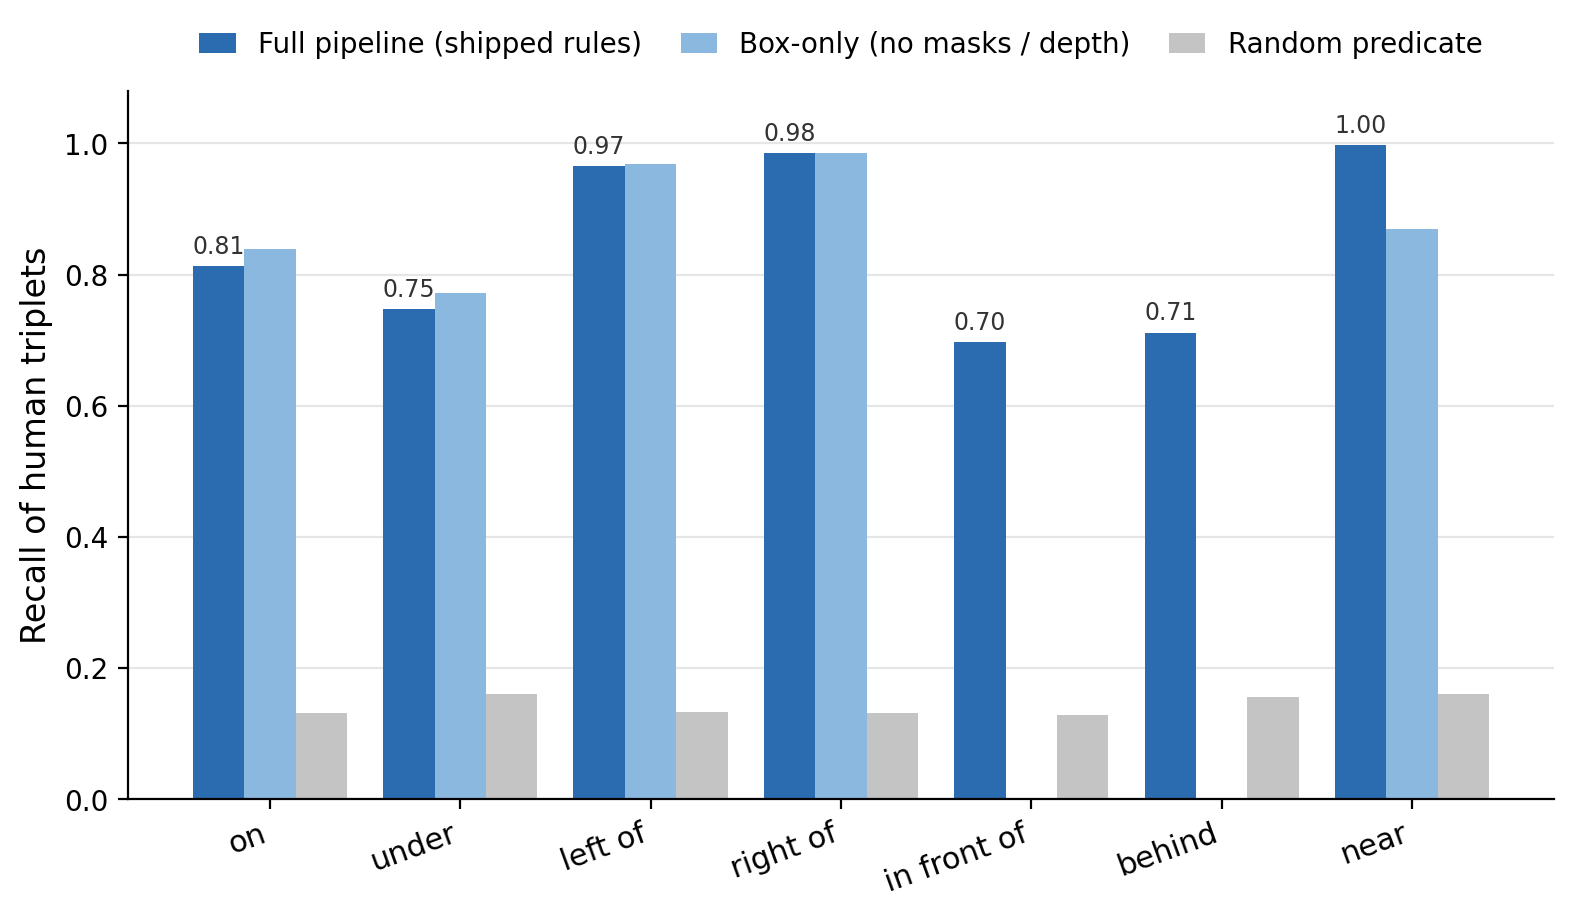
\includegraphics[width=0.95\textwidth]{figures/rq1-recall.png}
\caption{Recall of the human triplets per predicate: the full pipeline against a box-only ablation and a random baseline. Front and behind have no box-only bar because that ablation cannot compute depth.}
\label{fig:rq1-recall}
\end{figure}

\section{Precision on the annotated pairs}

\begin{center}
\small
\begin{longtable}{lrrrr}
\caption{Precision, recall and F1 restricted to the human-annotated pairs.}\\
\hline
Predicate & P & R & F1 & support \\
\hline
\endfirsthead
\hline
Predicate & P & R & F1 & support \\
\hline
\endhead
on & 0.88 & 0.88 & 0.88 & 1465 \\
under & 0.84 & 0.81 & 0.83 & 1001 \\
to the left of & 0.35 & 0.96 & 0.51 & 972 \\
to the right of & 0.42 & 0.98 & 0.59 & 1174 \\
in front of & 0.43 & 0.64 & 0.51 & 2013 \\
behind & 0.36 & 0.66 & 0.46 & 1584 \\
near & 0.12 & 1.00 & 0.21 & 717 \\
\hline
\end{longtable}
\end{center}

Restricted to the 8,790 human-annotated ordered pairs, precision is bounded below by construction: on an annotated pair the human typically recorded one or two relations, while several are geometrically true at once (a pair can be near, left-of and in-front-of simultaneously). The \texttt{near} row is the extreme case, since the tool emits \texttt{near} densely wherever the fitted gap threshold holds while only 3 of 9 annotator groups ever used the label, and it is exactly why the protocol includes the audit (\S4.4) rather than reading these columns at face value.

\subsection{Confusion: what the tool said when it missed}

For each human triplet the tool failed to recover, the labels it \textit{did} emit on that pair identify the failure mode directly:

\begin{center}
\small
\begin{longtable}{lrr}
\caption{For each missed human triplet, the predicates the tool emitted instead.}\\
\hline
Gold predicate & Missed & Most frequent co-emissions on missed pairs \\
\hline
\endfirsthead
\hline
Gold predicate & Missed & Most frequent co-emissions on missed pairs \\
\hline
\endhead
on & 177/1465 & near (177), behind (155): support demoted to proximity/depth \\
under & 187/1001 & in front of (167), near (166) \\
to the left of & 34/972 & near (33), to the right of (24): flips at the centre band \\
to the right of & 18/1174 & to the left of (16) \\
in front of & 725/2013 & near (572), behind (422), to the left of (261) \\
behind & 546/1584 & near (421), in front of (353) \\
near & 2/717 & on (2): the contact-exclusion boundary \\
\hline
\end{longtable}
\end{center}

Two structural signatures stand out. Missed front/behind pairs carrying the \textit{opposite} direction (422 + 353) are almost entirely the convention-inverted groups of \S4.5, and their count \textit{rose} with the ground-plane fallback, because pairs the tool used to abstain on are now committed in the direction those groups invert. And the two remaining missed \texttt{near} pairs carry \texttt{on}/\texttt{under}: the two rules disputing the contact boundary, the same support-rule frontier the audit (\S4.4) identifies from the precision side.

\begin{figure}[htbp]
\centering
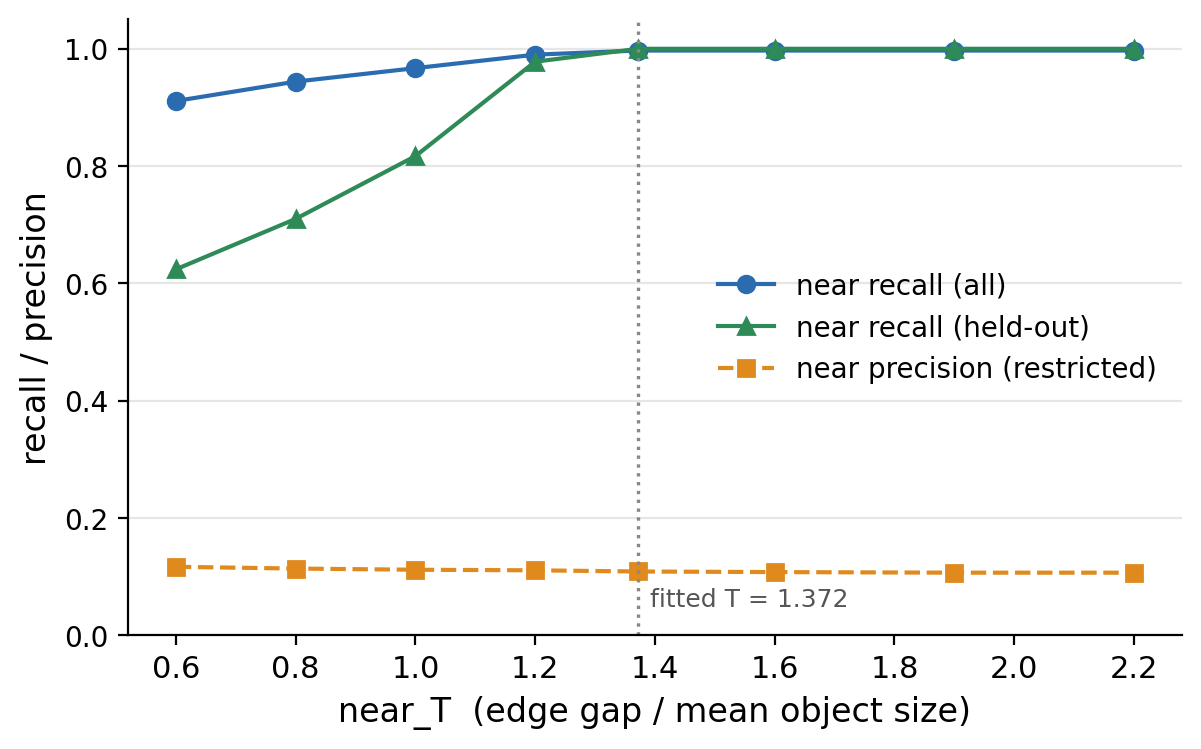
\includegraphics[width=0.95\textwidth]{figures/near-T-sweep.png}
\caption{Fitting the \texttt{near} threshold. Recall against all annotators and against the held-out annotator, with restricted precision. The fitted value is the tightest threshold at the plateau.}
\label{fig:near-T-sweep}
\end{figure}

\section{Manual audit of extra predictions (true-precision estimate)}

105 extra predictions (15 per predicate, seeded stratified sample) were rendered with subject/object boxes and manually verdicted, using a conservative rule under which any case not clearly true was marked wrong (\texttt{outputs/audit/audit\_sheet.csv}; verdicts to be independently spot-checked). This audit was run against the \textit{pre-gate box rule} and is reported as found because it motivated the support-rule repairs; \S4.9 re-audits the shipped rules (support precision \textasciitilde{}0.27 $\rightarrow$ \textasciitilde{}0.9), so the support rows below describe a fixed failure, not the final tool.

\begin{center}
\small
\begin{longtable}{lrrr}
\caption{Manual audit of a stratified sample of extra predictions, with Wilson intervals.}\\
\hline
Predicate & Correct / n & Precision est. & Wilson 95\% CI \\
\hline
\endfirsthead
\hline
Predicate & Correct / n & Precision est. & Wilson 95\% CI \\
\hline
\endhead
on & 1 / 15 & 0.07 & [0.01, 0.30] \\
under & 3 / 15 & 0.20 & [0.07, 0.45] \\
to the left of & 15 / 15 & 1.00 & [0.80, 1.00] \\
to the right of & 15 / 15 & 1.00 & [0.80, 1.00] \\
in front of & 15 / 15 & 1.00 & [0.80, 1.00] \\
behind & 15 / 15 & 1.00 & [0.80, 1.00] \\
near & 15 / 15 & 1.00 & [0.80, 1.00] \\
\hline
\end{longtable}
\end{center}

The audit splits the predicates cleanly in two. For the lateral, depth and proximity predicates, \textbf{every sampled extra prediction was correct}: the low restricted precision in \S4.3 is an artefact of sparse human labelling, exactly as the protocol anticipated, and the tool's dense labels on unannotated pairs are (within the sample's confidence bounds) trustworthy. For the support pair the picture inverts: extra \texttt{on}/\texttt{under} labels are mostly \textbf{false fires}. The box-adjacency test triggers on objects that merely project next to each other in clusters (a book \textit{behind} a bottle, a cube on the floor with a remote lying in front). Combined with \S4.2's containment misses, both error directions of the support rule point to the same repair, a mask-contact test instead of box adjacency, which the ablations evaluate. Two honest caveats: the sample is 15 per predicate, so per-predicate estimates carry wide intervals; and depth verdicts on near-coincident objects were occasionally marginal (noted in the sheet).

\section{The front/behind decomposition: a second measured annotation defect}

\begin{center}
\small
\begin{longtable}{lrrrrrr}
\caption{Front/behind by annotator group: emission rate, agreement where the tool commits, and the effect of aligning the direction convention.}\\
\hline
Group & Gold & Emit rate & Agreement when committed & Convention & Raw recall & Aligned recall \\
\hline
\endfirsthead
\hline
Group & Gold & Emit rate & Agreement when committed & Convention & Raw recall & Aligned recall \\
\hline
\endhead
group\_0 & 724 & 0.92 & 0.95 & same & 0.88 & 0.88 \\
group\_1 & 639 & 0.98 & 1.00 & same & 0.98 & 0.98 \\
group\_2 & 351 & 0.58 & 1.00 & same & 0.58 & 0.58 \\
group\_3 & 258 & 0.54 & 0.98 & same & 0.53 & 0.53 \\
group\_4 & 65 & 1.00 & 0.57 & same & 0.57 & 0.57 \\
group\_5 & 371 & 1.00 & 0.99 & same & 0.98 & 0.98 \\
group\_6 & 415 & 0.98 & \textbf{0.05} & \textbf{inverted} & 0.05 & 0.93 \\
group\_7 & 330 & 0.90 & 1.00 & same & 0.90 & 0.90 \\
group\_8 & 444 & 0.73 & \textbf{0.02} & \textbf{inverted} & 0.01 & 0.71 \\
\textbf{overall} & 3597 &  &  &  & \textbf{0.65} & \textbf{0.84} \\
\hline
\end{longtable}
\end{center}

(The table reports the shipped cascade, depth ordering plus the ground-plane fallback of \S4.9; the fallback roughly doubled the emit rates of the abstention-heavy groups 2 and 3.) The pooled 0.65 decomposes into three distinct causes:

\begin{enumerate}
\item \textbf{Direction agreement is near-perfect where the tool commits.} For six of
the eight groups with meaningful counts, agreement \textit{when a direction is emitted} is 0.95--1.00. Genuine depth-ordering errors are rare.
\item \textbf{Two annotator groups used the inverted convention.} Groups 6 and 8 agree
with the committed direction 2--5\% of the time; flipping their labels recovers 0.93/0.71. After the \texttt{near} findings, this is a \textit{second}, independent, measured annotation-consistency defect in the dataset: the direction convention for in front of/behind was not applied uniformly across annotators. This is the reference-frame ambiguity RoboSpatial formalises (\S2.5) observed in the wild: with no frame declared in the guidance, two annotator teams resolved it in opposite directions. (Aligned overall recall: 0.84. Alignment uses one disclosed bit per group, the majority direction of that group's own labels.)
\item \textbf{The remaining gap is abstention, not error.} Groups 2 and 3 agree with
the tool almost perfectly when it commits, but their scenes place object pairs inside the \texttt{depth\_eps} ambiguity band \textit{and} out of the ground-plane fallback's reach (elevated objects, near-tied bottom edges), so the tool abstains (emit rates 0.58 and 0.54, roughly doubled by the fallback from 0.30 and 0.08). The \texttt{depth\_eps} and \texttt{plane\_band} sweeps in the ablations trade this abstention against precision explicitly.
\end{enumerate}

\begin{figure}[htbp]
\centering
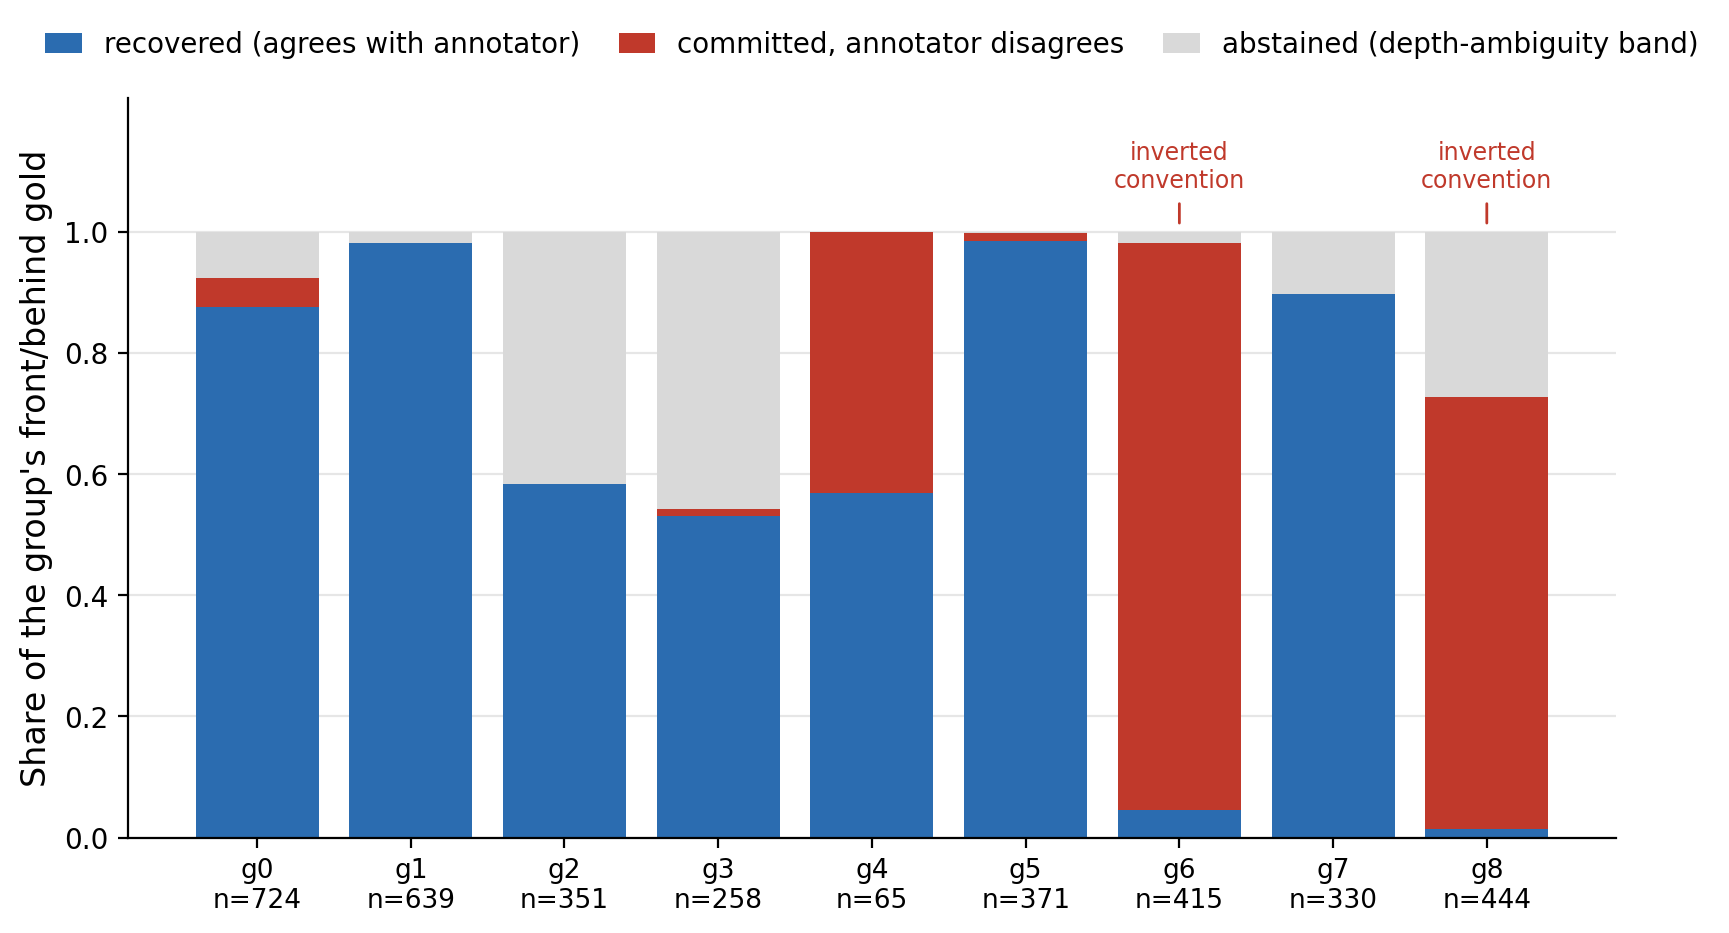
\includegraphics[width=0.95\textwidth]{figures/front-behind-decomposition.png}
\caption{Front/behind decomposed per annotator group: agreement where the tool commits, deliberate abstention, and the two groups that used the inverted direction convention.}
\label{fig:front-behind-decomposition}
\end{figure}

\section{The tenth annotator, and what the annotators would score against each other}

Per-group recall of each annotator's triplets (all predicates): group\_0 0.87 · group\_1 0.93 · group\_2 0.86 · group\_3 0.72 · group\_4 0.87 · group\_5 0.93 · group\_6 0.58 · group\_7 0.91 · group\_8 0.57. The dispersion is driven almost entirely by the two convention-inverted groups (6, 8): the tool agrees with the \textit{consistent} annotators at 0.72--0.93 (0.86--0.93 outside the abstention-heavy group 3).

On the held-out annotators specifically, the cluster-bootstrap intervals of \S4.2 are: on 0.922 (0.891--0.951), under 0.922 (0.879--0.960), left 0.953 (0.937--0.970), right 0.985 (0.974--0.996), near 1.000 (1.000--1.000), against in front of 0.197 (0.147--0.255) and behind 0.347 (0.281--0.417). Five of the seven predicates generalise to unseen annotators with intervals entirely above 0.87; the two depth predicates are separated from them by a gap far wider than the sampling uncertainty, which is what makes the convention explanation below a claim about the labels rather than about noise.

Reading those numbers as a quality verdict requires a yardstick the dataset does not supply: how well would two \textit{human} annotators agree with each other? The groups labelled disjoint image batches, so the quantity cannot be measured directly, and that absence is itself a finding about the dataset's construction. Two things can nevertheless be recovered by treating the automatic annotator as a fixed common reference (\texttt{eval/annotator\_agreement.py}).

\textbf{Annotator heterogeneity, measured without assumptions.} The tool is deterministic: it is literally the same labeller for every group, applying one definition. Any variation in its agreement across annotators is therefore variation in the \textit{annotators}. Across the seven consistent groups that variation spans 0.717 to 0.933, a spread of 0.216 (sd 0.068). Before any inference about human-human agreement, this alone establishes that the annotators are not interchangeable, and it puts a number on how far apart they are.

\textbf{Bounds on human-human agreement.} For any common reference, if annotator A agrees with it on a fraction p\_A of items and B on p\_B, their mutual agreement p\_AB obeys the Fréchet inequalities max(0, p\_A + p\_B − 1) $\leq$ p\_AB $\leq$ 1 − |p\_A − p\_B|. Averaged over all 21 pairs of consistent annotators, these place annotator-to-annotator agreement in \textbf{[0.74, 0.92]}. The tool's own mean agreement with those annotators, \textbf{0.869, lies inside that interval}. In other words, the automatic annotator agrees with the human annotators about as well as the evidence permits them to agree with each other. One assumption is required and is stated rather than buried: because the batches are disjoint, the bounds presume each annotator's agreement rate would carry over to another \textasciitilde{}100-image batch. The interval is therefore an estimate, not a measurement, and the independent validation study (\S4.13) is what tests the underlying precision claim without it.

\section{Flags: the honest human cost}

31.5\% of ordered pairs carry a flag: depth-ambiguous 19.3\% (down from 29.5\% before the ground-plane fallback, which resolved a third of the depth abstentions) and lateral-ambiguous 10.0\% are \textit{abstentions} (no label emitted; nothing to review), while the borderline-near band, 8.5\% of pairs, is the genuine review queue. At a conservative 3 seconds per queued pair this is $\approx$6 hours of review for the full dataset, versus the original nine-annotator manual pass. And it is optional, not required, for the fidelity reported above.

\subsection{The missing guidelines, confirmed at the source}

The annotation guidance the annotators worked from (confirmed from the SGDET-Annotate repository the supervisor indicated) consists of vocabulary lists only, object names and 19 relationship terms, with no operational definitions. Every annotator behaviour this chapter measures (the selective use of \texttt{near}, the inverted front/behind convention, one-directional support labelling) is the predictable consequence of labelling with undefined terms, the exact failure mode the annotator-disagreement literature documents across vision and language tasks (\S2.3). The geometric specification of Chapter 3 is therefore not a re-implementation of existing rules but the first operational definition of these predicates, and the fitted thresholds are exactly the "clear annotation guidelines" the source paper's future work requests.

\section{Answer to RQ1}

Automated annotation reaches human-comparable quality on six of seven predicates outright (0.81--1.00 recall of the human triplets; mean 0.85, with 0.76 on annotators no threshold ever saw), matches the human notion of \texttt{near} completely once the label's inconsistent usage is accounted for (0.997 pooled, 1.00 held-out at the fitted threshold), resolving the one predicate the source paper reports as failing for every model it benchmarks (\S2.2). On the depth pair, after the depth-plus-ground-plane cascade, it recalls 0.64/0.66 pooled and agrees with every consistently-labelled annotator 95--100\% of the time where it commits; aligned for the two inverted-convention groups, depth recall is 0.84. The remaining shortfall decomposes, in measured proportions, into calibrated abstention and that inverted convention. The audits bound true precision: \textasciitilde{}1.0 for the lateral and proximity predicates and for depth-decided front/behind, \textasciitilde{}0.9 for support after the contact rule, and \textasciitilde{}0.73 conservative for the ground-plane fallback's added commits (\S4.9). The tool's residual cost is the \textasciitilde{}8\% borderline review queue, and its labels are 20$\times$ denser than the human set.

\section{Shipped from the ablations}

Four rule changes came out of the audit-and-ablation loop; each is reported with its calibration, its held-out validation and its audit.

\subsection{The support depth-co-location gate}

The audit's support-precision failure has a geometric cause: on a floor plane, "farther" projects as "higher in the image", so a behind-pair produces the same 2D box signature as a stacked pair. The repair is a depth co-location condition on \texttt{on}/\texttt{under} (truly stacked objects share a camera distance), an instance of the reject-the-geometrically-impossible correction principle adapted from Open3D-VQA (Zhang et al., 2025; \S2.5), calibrated on the train groups (\texttt{on\_depth\_eps} = 0.06) and validated held-out (ablation A1): support F1 on never-seen annotators rises 0.58 $\rightarrow$ 0.71. Downstream effects on the headline table: support recall −2/−3 points, \texttt{on} restricted precision 0.57 $\rightarrow$ 0.73, 44\% fewer support emissions (of the 26 audited false positives, the gate removes 12 while keeping all 4 true positives), and, because fewer false contacts suppress fewer proximity labels, \texttt{near} recall rises 0.87 $\rightarrow$ 0.95 (held-out 1.00). Mean recall is unchanged at 0.79 with a substantially more trustworthy label set. The residual false fires are same-depth cluster neighbours, which depth cannot separate by construction; they are addressed next.

\subsection{The mask-contact rule}

The support signature that boxes cannot see, masks can: A rests on B iff the pixels directly below A's mask-bottom boundary belong to B (\texttt{src/contact.py}), which captures both stacking and the containment case, and rejects side-by-side neighbours. Calibrated on the train groups (\texttt{on\_contact\_min} = 0.60; the train-F1 plateau is flat from 0.60--0.80, so the choice is uncritical), ablation A5: support F1 on held-out annotators rises again, 0.71 $\rightarrow$ \textbf{0.87}, with \texttt{on} recall 0.82 $\rightarrow$ 0.88 and restricted precision 0.73 $\rightarrow$ 0.88 simultaneously, the rare change that improves both error directions at once, exactly as the failure gallery and audit predicted. Knock-on: \texttt{near} recall reaches \textbf{0.997 pooled (715/717; the two residual misses are contact-boundary cases, \S4.10) and 1.00 held-out} as the last contact-boundary suppressions disappear; headline mean recall 0.79 $\rightarrow$ \textbf{0.81}. The A4 sweep confirms the fitted threshold sits exactly at the recall plateau's knee: recall is flat from T = 1.372 upward while emissions keep growing, so the fitted value is the least-permissive point achieving maximal agreement. A 30-sample re-audit of the new support extras confirms the precision claim independently: extras correct rise from 1/15 and 3/15 (box rule) to \textbf{11/15 and 12/15}, an estimated true support precision of \textasciitilde{}0.27 $\rightarrow$ \textasciitilde{}0.9. The seven remaining wrong/uncertain extras have structure: a person \textit{holding} a remote fires contact (holding ≠ resting), one occluded bottle-behind-bottle pair, and three distant clusters too small to verdict confidently. The person-holding mode is closed by a \textbf{class-aware guard}: annotators never label person-support (0 of 2,466 gold support triplets involve a person on either side), so \texttt{on}/\texttt{under} are simply not evaluated for that class, removing \textasciitilde{}130 false emissions at no recall cost, since the person side carried no gold to recover.

\subsection{The ground-plane fallback}

The depth abstention band was the single largest miss cause, and most of it is resolvable without depth at all: two objects standing on the same floor are depth-ordered by pure projection. The nearer object's box bottom sits lower in the image, a pixel-precise cue exactly where relative depth is noisiest. The shipped rule fires only where the depth rule abstained, only when \textit{neither} object rests on another object by the tool's own contact evidence (an elevated object's box bottom locates its support, not itself), and only outside a small bottom-edge band (\texttt{plane\_band} = 0.005, calibrated on the train groups; ablation A7). On the train groups the fallback adds 386 committed directions at 0.91 agreement; on held-out group 7 it adds 54 and \textbf{every one agrees with the annotator}. Effect on the headline: front/behind recall 0.52/0.55 $\rightarrow$ \textbf{0.64/0.66} (aligned overall 0.67 $\rightarrow$ \textbf{0.84}), mean recall 0.81 $\rightarrow$ \textbf{0.85}, and the depth-ambiguous flag rate falls 29.5\% $\rightarrow$ 19.3\%. A seeded 15-sample audit of the fallback's \textit{extra} predictions (pairs no human labelled) estimates true precision conservatively at \textbf{11/15 $\approx$ 0.73}, and the four wrong/uncertain cases share one structure: an object resting on something the detector has no box for (a book on an unannotated case; a stacked-book pair whose contact fell below threshold), i.e. elevation the guard cannot see. That residual mode is documented, bounded, and exactly the undetected-support refinement the support audit already motivates.

\subsection{Follow-up refinements: one shipped, two declined}

The class-aware guard \textit{shipped}: annotators never label person-support (0 of 2,466 gold triplets), so support is no longer evaluated when either object is a person, removing \textasciitilde{}130 held-object emissions at zero recall cost and eliminating the person-holding audit mode by construction. Two further candidates were built, measured, and rejected on the evidence. (i) \textit{Guard-only surface detection} (zero-shot prompts for tables, cases and trays feeding the elevation guard; \texttt{scripts/run\_surface\_guard.py}) suppressed 6\% of the fallback's extra commits at a cost of 0.01 behind recall, but blocked none of the four audited failures, whose supports are either annotated-class objects with below-threshold contact (flat stacked books) or surfaces the detector missed; the machinery and its cache are retained as an ablation (\texttt{outputs/surface\_guard\_ablation/}). (ii) \textit{A larger depth model} (Depth Anything v2 Base, 4$\times$ the parameters) moved front/behind recall by +0.001/+0.002: the remaining depth ambiguity lives in the scenes, not in model capacity, and the Small variant's Apache licence is kept. Both null results bound where further engineering can and cannot help.

\subsection{Why a geometric cue, not a bigger depth model (ablation A8)}

It is worth asking whether the depth pair would improve simply by using a stronger depth network. It does not: swapping Depth Anything v2 Small for the 4$\times$ larger Base variant and re-running the whole dataset moves front/behind recall by +0.005 (0.636/0.652 $\rightarrow$ 0.641/0.656) and mean recall by +0.000. The depth-predicate limit is \textit{monocular ambiguity} (two objects at a similar camera distance are inseparable by any monocular model, regardless of its fidelity), not the network's quality. This is precisely why the fallback that worked is a geometric projection cue rather than a heavier perception model, and it justifies shipping the Small variant: identical accuracy, an Apache-2.0 licence, and half the VRAM.


\section{Failure gallery: every miss diagnosed}

Each missed human triplet is diagnosed automatically by re-checking the rule's individual conditions against the cached geometry and mask-contact maps (\texttt{scripts/make\_failure\_gallery.py}; rendered examples in \texttt{outputs/failure\_gallery/}). With the shipped rule set (1,689 misses):

\begin{center}
\small
\begin{longtable}{ll}
\caption{Diagnosed cause of every missed human triplet, by predicate.}\\
\hline
Predicate & Dominant causes (share of that predicate's misses) \\
\hline
\endfirsthead
\hline
Predicate & Dominant causes (share of that predicate's misses) \\
\hline
\endhead
in front of & abstained in ambiguity band 61\% · convention-inverted annotators 38\% · \textbf{genuine depth error 1\%} \\
behind & abstained 52\% · convention-inverted 42\% · \textbf{genuine depth error 5\%} \\
on & mask contact below threshold 58\% · depth-gate suppressed 40\% \\
under & contact below threshold 50\% · depth-gate suppressed 33\% · no contact measured (occlusion) 17\% \\
near & 2 remaining misses (contact boundary) \\
to the left/right of & centre flip 71--89\% · abstained 11--29\% (52 cases total) \\
\hline
\end{longtable}
\end{center}

Genuine depth-ordering errors remain 1--5\% of front/behind misses; the support misses are threshold/gate trades on real contact evidence rather than box-geometry artefacts; and \texttt{near} misses have all but vanished. The convention-inverted \textit{share} grew (38--42\%, from 28--32\%) not because those misses increased but because the ground-plane fallback shrank the abstention share around them; total misses fell from 2,107 to 1,689. Misses attributable to avoidable tool error across all seven predicates: \textasciitilde{}7\%.


\section{Detector-in-the-loop: full automation, attributed}

The deployment mode replaces ground-truth boxes with Grounding DINO (Liu et al., 2024) zero-shot detection (short-noun text prompts for the six classes; threshold 0.25, tuned in one disclosed iteration on a 20-image trial), then runs the identical SAM2 $\rightarrow$ depth $\rightarrow$ rules stack (\texttt{scripts/run\_sgdet.py}, scored by \texttt{eval/sgdet\_eval.py} with class-matched greedy IoU $\geq$ 0.5).

End-to-end triplet recall over all 836 images is \textbf{0.38} against the PredCls headline, and the decomposition attributes the gap exactly. Zero-shot detection recall spans 0.40 (cube) to 0.95 (human), and a triplet needs \textit{both} endpoints found. \textbf{Conditioned on both endpoints being detected, the relation layer scores 0.85 mean, matching its PredCls performance} (lateral 0.96/0.98, near 1.00, support 0.83/0.77; front/behind 0.69/0.70, computed before the ground-plane fallback shipped, so the conditional depth numbers are a floor; detectable pairs also skew towards well-separated objects). The gap is therefore entirely a detection problem, not a relations problem: the geometric rules are detector-agnostic.

Two honest notes. Zero-shot open-vocabulary detection is the worst-case detector, exactly the reach-versus-per-class-recall trade \S2.6 identifies, and it was used because the authors' trained YOLOv10m weights (0.93 mAP@50 in the source paper) were not available; with that detector the end-to-end gap would largely close. And the 20-image trial over-estimated detection quality (its scenes come from one annotator batch), a reminder that the full-set numbers are the ones that matter.

\section{Video demonstration}

Two short royalty-free stock clips (sources in Appendix A) were processed per frame by the deployment-mode stack of \S4.11 with open-vocabulary prompts, greedy IoU tracking for stable object identities, and a $\pm$2-frame temporal majority vote over each pair's predicates (\texttt{scripts/run\_video.py}; overlays and per-frame records in \texttt{outputs/video/}). The clips were chosen as complementary regimes: a \textbf{moving camera over a static desk scene} (clip 1, 99 processed frames), where relations should stay constant and any variation is measurement noise; and a \textbf{static overhead camera with moving hands} (clip 2, 79 frames), where relations genuinely change and smoothing must not erase the change.

Three observations. \textbf{(i) Relations are stable wherever identity is stable.} For object pairs co-visible in $\geq$20 frames, the emitted predicate persists at 0.90/0.94 mean across the two clips, with 81\% and 89\% of pair-predicates present in $\geq$90\% of their co-visible frames (\texttt{eval/video\_stability.py}, which derives these from the recorded per-frame files; co-visible means both track identities appear in that frame). The temporal vote is what separates the two clips: it lifts persistence from 0.896 to 0.902 on the static-scene clip and from 0.915 to 0.938 on the one with moving hands, which is the clip where per-frame detection actually churns. Frame-to-frame triplet agreement (Jaccard 0.89 for clip 1, 0.70 for clip 2) is dominated by zero-shot detection churn and, in clip 2, genuine hand motion; the dips in the stability trace align with the hands picking objects up. This mirrors \S4.11's attribution exactly: the variation is detection, not relations. \textbf{(ii) The rules transfer to objects they were never calibrated on}: the pen resting on the notepad and a wallet-and-photograph stack are labelled with the same contact evidence fitted on the dataset's six classes. \textbf{(iii) The camera-frame semantics are visible}: in the bird's-eye clip, in front of/behind re-maps to distance from the viewer's edge of the desk, the reference-frame dependence \S2.5 cites from RoboSpatial, demonstrated rather than asserted. The open-vocabulary quirks are equally visible and worth recording: content displayed \textit{on the laptop's screen} is detected as real objects, and items outside the prompt list snap to the nearest prompted class (an earbuds case becomes a \texttt{cup}).

This is a demonstration, not an experiment (no video ground truth exists), but it establishes that the annotator is video-ready at \textasciitilde{}2--3 s per frame, with SAM2's native mask propagation (it is a video model used here frame-wise) as the designed upgrade path for true temporal consistency.

\textbf{It is also the project's only out-of-domain evidence, and worth reading as such.} The clips share nothing with the dataset the rules were calibrated on: different scenes (an office desk and an overhead worktop, not a laboratory floor), a different camera and viewpoint, and objects drawn almost entirely from outside the six annotated classes (a monitor, keyboard, mouse, mug, spectacles, potted plants, a lamp, a notepad, a laptop, a cactus, a wallet, photographs, an earbuds case). No threshold was retuned: \texttt{near\_T}, the depth band, the contact fraction and the plane band are the values fitted on annotator groups 0--5 of the robot dataset. The support relations that emerge (a pen resting on a notepad, a wallet-and-photograph stack) are decided by the same mask-contact evidence, and the camera-frame semantics behave exactly as the design predicts when the viewpoint changes to bird's-eye.

The limits of that evidence should be equally clear: with no ground truth these are qualitative judgements over two clips, so they support the claim that the \textit{rules} carry to new object types and viewpoints, and they say nothing quantitative about accuracy in a new domain. A labelled cross-domain sample is the measurement this substitutes for, and it remains future work (\S7.6). What the clips do settle is that transfer is not blocked by the object vocabulary: the failures visible in them are detection failures (screen content detected as real objects, unprompted items snapping to the nearest prompted class), which is the same attribution \S4.11 makes for the dataset itself.

\begin{figure}[htbp]
\centering
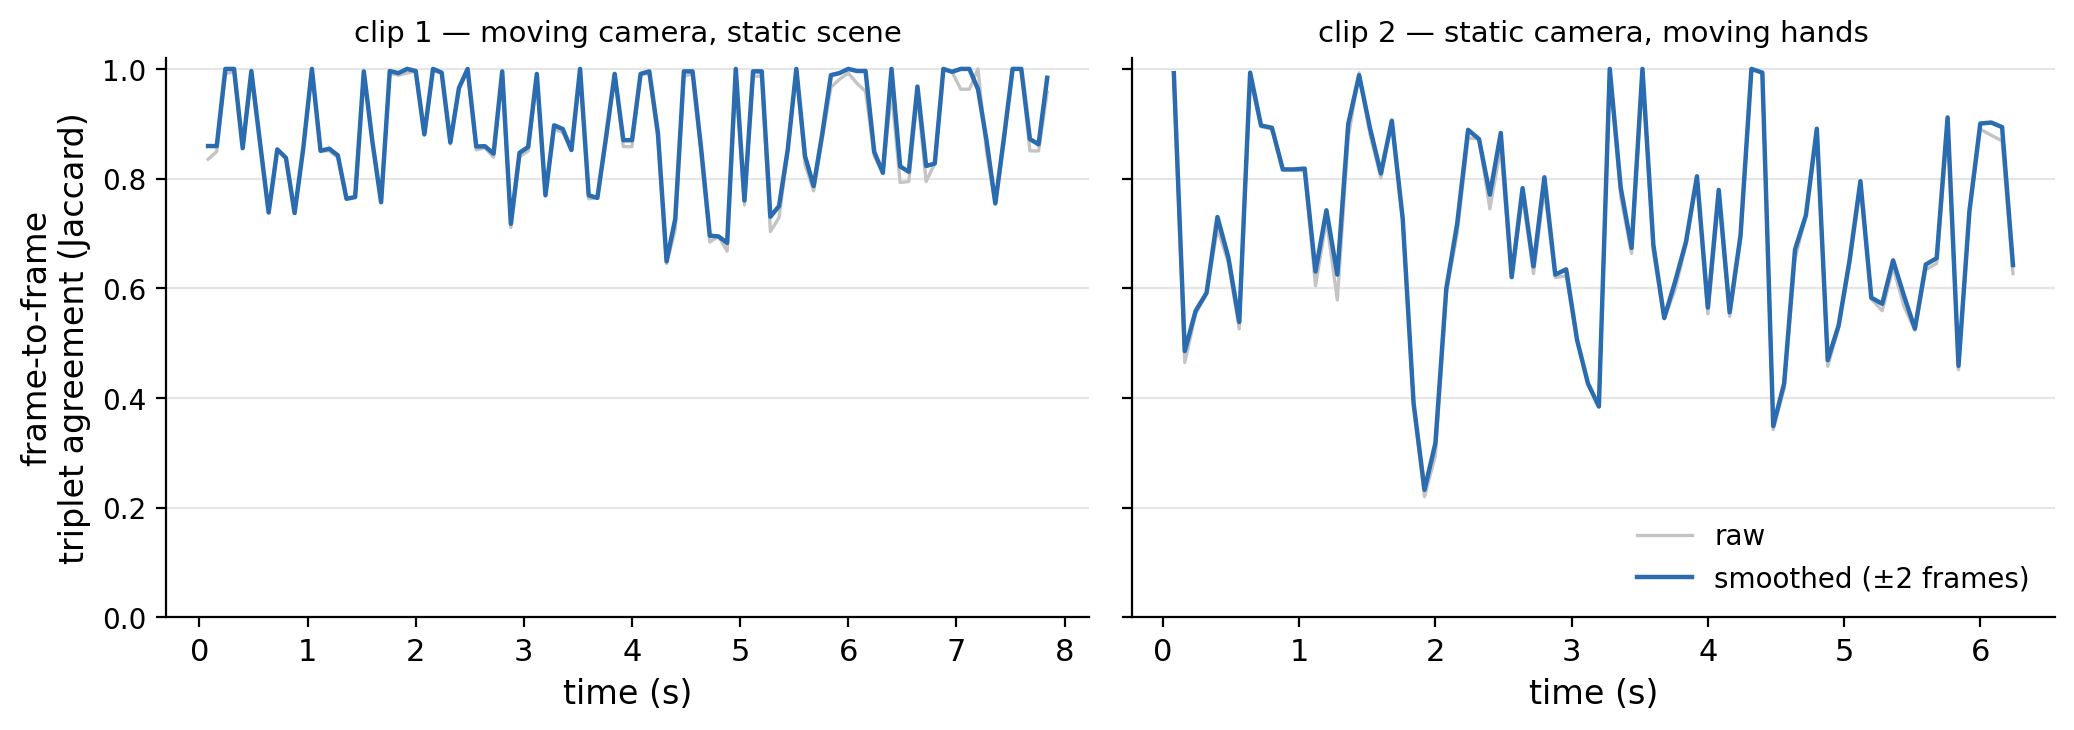
\includegraphics[width=0.95\textwidth]{figures/video-stability.png}
\caption{Frame-to-frame stability of the emitted triplets on the two demonstration clips, before and after temporal smoothing.}
\label{fig:video-stability}
\end{figure}

\section{Independent validation of the precision estimate}

The true-precision estimates of \S4.4 and \S4.9 have one methodological weakness that no amount of sampling fixes: they were verdicted by the author of the tool being evaluated. Conservative rules and published evidence mitigate the risk, but they do not remove it, and the honest description of those numbers is "author-verdicted". A separate study was therefore designed to re-estimate precision with judges who have no stake in the result.

\textbf{Protocol.} A stratified sample of 2,002 automatic labels (286 per predicate) is drawn from the tool's \textit{extra} predictions, meaning ordered pairs the human annotators never labelled, which is exactly the population with no ground truth to score against. Each claim is rendered as the source photograph with the subject outlined in red and the object in blue, and presented with a single sentence ("the book is on the box") to volunteers recruited by open link, who answer TRUE or WRONG / can't tell. The instructions restate the operational definitions of Chapter 3: camera-frame laterality, "in front of" as nearer the camera, support as physically resting rather than held, and an explicit instruction to answer WRONG when unsure, which reproduces the conservative rule used in the author's audits. Each browser receives a random identifier that prevents repeat judgements without identifying anybody, and faces are anonymised in every image (Chapter 8).

Coverage is stratified by what each analysis requires. An aggregate precision estimate needs only one judgement per claim, since the sample is random either way, so ordinary claims target a single rater. The 147 claims that also carry an author verdict target three raters each, because the crowd-versus-author comparison and the inter-rater reliability figure both need several independent judgements on the \textit{same} item; those claims are served first. The design therefore needs about 2,300 judgements rather than the 6,000 a uniform three-rater target would demand, and it fails gracefully: the author-comparison subset completes after roughly 30 participants, so that analysis survives a thin turnout while any further response widens the precision estimate.

\textbf{What it measures.} Three things the author-verdicted audits cannot. First, crowd precision per predicate with binomial confidence intervals, at a sample size two orders of magnitude larger than the n = 15 per predicate of \S4.4. Second, an author-bias check: the 147 items carrying the author's own verdicts are retained inside the pool, so crowd majority and author verdict can be compared directly by percentage agreement and Cohen's kappa (Cohen, 1960). Third, whether the \textit{task} is well posed at all, through crowd-internal reliability across raters (Krippendorff's alpha), which distinguishes "the tool is wrong" from "this claim is genuinely ambiguous", a distinction the annotator-disagreement literature insists on (\S2.3).

Scoring is fully specified in advance (\texttt{analysis/score\_votes.py}): ties resolve to WRONG, matching the audit protocol; reflex-speed responses and raters who disagree systematically with everyone else can be excluded by pre-declared filters. The instrument is complete and collection is under way; the results are reported at submission, and the limitation stated in \S7.4 stands until they are.

\section{Temporal redundancy and stability under viewpoint change}

The 884 released images are not independent photographs. Pixel-matching them against the 2,650-frame raw capture the supervising group later supplied identifies them exactly: they are frames 000000--000883 of one continuous walk, and each annotator group is a contiguous 100-frame block (\texttt{group\_0} = frames 0--99, \texttt{group\_1} = 100--199, and so on). This has two consequences, one methodological and one that yields a measurement the rest of the chapter cannot make.

\textbf{The methodological one first, because it qualifies earlier results.} A group is simultaneously an annotator identity \textit{and} a temporal block holding one arrangement of objects. The held-out split of \S4.1 is therefore held out by annotator \textit{and} by scene, not by annotator alone as described. The annotator reading survives, since a systematically inverted front/behind convention (\S4.5) and a \texttt{near} label used by three groups in nine (\S3.2) are properties of labelling behaviour, and no arrangement of furniture can produce them, but the held-out figures carry a domain shift alongside the annotator shift. The direction of that confound is favourable, in that 0.76 on held-out groups is generalisation to an unseen annotator \textit{and} an unseen arrangement, which is the harder of the two readings; it is recorded here because the design was described as one thing and the data supports a slightly stronger one.

\textbf{The measurement.} Because the frames are consecutive, a scene appears repeatedly from different viewpoints, and the pipeline's verdicts can be compared across those viewpoints without any human labels. The comparison is a reliability test of a kind sparse human annotation cannot supply: a relation determined by geometry should survive the camera moving, and one decided by a coin-toss at a decision boundary should not.

Frames were segmented by content drift (\S3.10) and each segment's predicates propagated from its keyframe to the remaining frames, matching objects by class and box overlap because object indices are not stable across frames: the annotators recorded different subsets of the scene from frame to frame, and \texttt{group\_0} alone contains 43 distinct object orderings (\texttt{eval/keyframe\_propagation.py}).

\textit{Segmentation.} At τ = 10 the full 2,650-frame sequence collapses to 892 segments, a 3.0$\times$ reduction; over the 884 released frames alone it gives 331 segments, 2.7$\times$. Scored on that released portion, where the eight layout changes are known, every one is recovered within five frames (boundary recall 1.00). Precision against those eight is low by construction and not a defect: viewpoint changes within a block are genuine content changes, merely finer-grained than the layout changes.

The comparison worth recording is with the standard alternative. Thresholding consecutive-frame differences, the basis of shot detection, does not merely perform worse here, it has no usable operating point at all. At a threshold of 15 grey levels it fires 13 times across the annotated frames and finds none of the eight; lowering it to 5 finds all eight but among 604 firings, a precision of 0.013, and lowering it further only adds firings. There is no setting at which the layout changes separate from the noise, because the per-step signal they produce is not larger than the noise; only the accumulated drift is.

\textit{Stability and cost.} The propagation runs over the 802 annotated frames that carry pair records, segmented within each group so no segment straddles two arrangements. At τ = 10 that yields 568 keyframes, leaving 234 frames whose predicates are propagated rather than computed, and 11,352 object pairs on which the two can be compared. (The compression here is lower than the 2.7$\times$ quoted above because these 802 frames are a subset of the sequence: consecutive members sit further apart in the original capture, so more drift accumulates between them.) The table below reports per predicate how often the keyframe's verdict matches what the pipeline computes on the frame directly, alongside recall of that frame's human triplets under propagation and under per-frame computation.

\begin{center}
\small
\begin{longtable}{lrrr}
\caption{Stability of each predicate across viewpoints of the same scene, with recall under keyframe propagation against per-frame computation.}\\
\hline
Predicate & Stability & Recall (propagated) & Recall (per frame) \\
\hline
\endfirsthead
\hline
Predicate & Stability & Recall (propagated) & Recall (per frame) \\
\hline
\endhead
on & 0.909 & 0.897 & 0.864 \\
under & 0.909 & 0.829 & 0.795 \\
to the left of & 0.989 & 0.959 & 0.966 \\
to the right of & 0.989 & 0.989 & 0.989 \\
in front of & 0.955 & 0.627 & 0.601 \\
behind & 0.955 & 0.601 & 0.613 \\
near & 0.966 & 1.000 & 1.000 \\
\textbf{Mean} & \textbf{0.953} & \textbf{0.843} & \textbf{0.832} \\
\hline
\end{longtable}
\end{center}

Skipping frames costs nothing measurable. Mean recall under propagation is 0.843 against 0.832 computed per frame, and the ordering holds at every threshold tested (0.879 against 0.861 at τ = 20, a 4.0$\times$ reduction). The small advantage is plausibly an artefact of the selection rule rather than a benefit of propagation: the segment representative is the frame nearest the segment mean, which on a moving camera is less likely to be caught mid-transition than an arbitrary frame.

\textbf{The finding that matters is in the first column, and it is not the one expected.} Front/behind was predicted to be the least stable predicate, on the assumption that its errors come from monocular depth noise near the decision boundary; noise of that kind should flip verdicts when the camera moves. It does not. Front/behind agrees with itself across viewpoint changes 0.955 of the time, above \texttt{on}/\texttt{under} at 0.909, and still 0.924 when the segmentation is coarsened to 89$\times$ compression, where segment members are substantially different views. A predicate whose recall against human labels is 0.60 while its agreement with itself across viewpoints is 0.96 is not making random errors. It is making the same call repeatedly and disagreeing with the annotators systematically.

That converges with two independent results. Ablation A8 (\S4.9) showed a depth model four times larger does not improve front/behind, which is what one expects if the limit is not depth resolution; and \S4.5 measured two annotator groups labelling the pair in the opposite direction, which is a disagreement about what the words mean. The viewpoint-stability figure adds the evidence those two could not: the tool's verdicts are reproducible under exactly the perturbation that would expose measurement noise. Monocular ambiguity remains a real bound on the predicate (\S9.3), but the gap between 0.64 and 1.00 on this dataset is dominated by definitional disagreement rather than by an unsteady depth estimate.

\textbf{Limits of this measurement.} Two, both restricting scope rather than direction. Stability is computed only on object pairs that could be matched between keyframe and frame, and those are pairs whose objects moved least in the image, which is plausibly the easier population; the figures are therefore an upper bound on stability over all pairs. And matched coverage falls sharply as segments grow, from 88.7\% of pairs at τ = 5 to 58.5\% at τ = 10 and 26.5\% at τ = 20, so aggressive compression leaves most pairs uncovered rather than mislabelled. The cause is box drift under camera motion rather than missing annotation: at τ = 20, 65\% of skipped frames carry an identical object count to their keyframe, and relaxing the overlap criterion from 0.5 to 0.1 cuts unmatched objects from 5.6 to 2.2 per frame. Carrying object identity with a tracker, which \texttt{scripts/run\_video.py} already does for video, rather than with per-frame overlap, is the change that would recover it, and it is a straightforward extension rather than a research question.

\section{Scale, measured rather than extrapolated}

Throughput and density elsewhere in this chapter are measured on the 836 annotated images, which leaves the claim that the method extends to new captures resting on an extrapolation. The 1,766 unannotated frames of the raw sequence (\S4.14, Appendix A) remove that gap: they are robot output nobody has labelled, from the same platform and laboratory but from later in the session, with arrangements and rooms the tool has never been shown.

No accuracy claim is available here, since there is no ground truth, and none is made. What the run establishes is operational, and there are three parts to it.

\textit{Cost.} Content-adaptive selection reduces 1,766 frames to 562 keyframes, 3.1$\times$. In deployment mode the pipeline sustains 3.33 s per frame on the RTX 2060 (1,080 frames per hour, JSON only; rendering an inspection overlay for every frame roughly doubles that). The keyframe pass therefore takes 31 minutes where annotating every frame would take 98.

\textit{Yield.} The run emits 185,242 triplets over 562 frames, 330 per frame from 11.7 detected objects. No frame produced an empty graph. For comparison, the human process recorded 8,926 triplets across 836 images, about 11 per image.

\textit{Behaviour.} The risk with unfamiliar input is not loud failure but quiet drift, a pipeline that keeps emitting labels whose distribution has silently changed. Compared against the same detector on the annotated images, the predicate distribution is close to unchanged: total variation distance 0.032, with the largest single shift 0.015 (in front of, 0.181 to 0.195). The \texttt{on}/\texttt{under} share is low in both runs, 0.006 annotated against 0.003 here, which is a property of open-vocabulary detection rather than of the new frames: more detected objects means more pairs, and most pairs are not in contact. Density per frame is lower than on the annotated portion (330 against 633 triplets) for the same reason in reverse, since the later arrangements hold fewer objects (11.7 detections against 16.9) and pair count grows with the square of that.

The honest summary is that the scaling claim now rests on a run rather than an argument, and that what it demonstrates is capacity and stability, not correctness. Establishing correctness on this portion needs labels that do not exist; the viewpoint-consistency measurement of \S4.14 is the closest available substitute, and it is a check on self-agreement rather than on truth.

\chapter{Downstream Utility (RQ2)}

\begin{quote}
Numbers generated by \texttt{eval/downstream.py} and, for \S5.7, by \texttt{eval/score\_planner.py}; reproducible from \texttt{outputs/rq2\_report.json} and \texttt{outputs/planner\_scores.json}.
\end{quote}

This chapter answers RQ2 with a controlled experiment over three label sources. Section 5.1 states the design, \S5.2 the result, \S5.3 examines why self-training fails to rescue the human labels, \S5.4 the mechanism and its consistency checks, \S5.5 the boundaries of the claim, and \S5.6 the connection to the source paper's robot-planning chain. Section 5.7 then tests that chain one link further, asking whether the label source changes the plan an LLM planner produces for a robot, and \S5.8 gives the answer.

\section{The controlled experiment}

RQ2 asks whether the automatic labels are good enough to \textit{train} a relation model as effectively as human labels. The experiment isolates exactly that variable: one lightweight classifier per predicate (a small MLP over pure geometric pair features: relative position, depth difference, box geometry, size-relative gap, mask-contact fractions), trained with \textbf{identical features, architecture, seed, positive-oversampling and group split}, then evaluated against the \textbf{held-out human gold} (annotator groups 6--8, whose data influenced no threshold, no calibration, and no training). The only difference between the runs is the supervision source. (Training uses a fixed 60-iteration budget for every classifier; some do not fully converge, identically for every source; the comparison is between supervision signals under equal compute, not between tuned models.)

Three sources are compared, because two would leave the obvious objection unanswered.

\begin{itemize}
\item \textbf{Human.} The \textasciitilde{}10\% of ordered pairs the annotators chose to label.
\item \textbf{Automatic.} Every pair the tool's rules fire on: dense and
rule-consistent.
\item \textbf{Self-trained (pseudo-labelled).} The rival remedy from the
semi-supervised literature (\S2.4), implemented rather than argued about. A teacher is trained on the human labels exactly as in the human arm; it then predicts the \textit{unannotated} training pairs, its confident predictions (probability $\geq$ 0.90 either way) become pseudo-labels, and a student is retrained on the union of real and pseudo labels (Lee, 2013). A pair the annotators touched at all counts as labelled, since their silence on its other predicates is informative; a pair they never recorded is the unlabelled pool. This arm answers the question a reader should ask before accepting the project's premise: if the human labels are too sparse, why not simply stretch them?
\end{itemize}

Each source labels the same pairs its own way, and each model inherits its source's character. That contrast is the experiment.

\section{Result}

Averaged over three seeds (42/43/44); each cell shows mean (min--max):

\begin{center}
\small
\begin{longtable}{lrrrr}
\caption{Downstream recall against held-out human gold for the three label sources.}\\
\hline
predicate & human-trained & self-trained & auto-trained & gold (held-out) \\
\hline
\endfirsthead
\hline
predicate & human-trained & self-trained & auto-trained & gold (held-out) \\
\hline
\endhead
on & 0.84 (0.83--0.86) & 0.90 (0.89--0.92) & 0.92 (0.92--0.93) & 348 \\
under & 0.44 (0.36--0.53) & 0.59 (0.59--0.60) & 0.92 (0.92--0.93) & 192 \\
to the left of & 0.22 (0.18--0.29) & 0.31 (0.27--0.34) & 0.95 (0.95--0.95) & 446 \\
to the right of & 0.25 (0.22--0.31) & 0.38 (0.37--0.39) & 0.99 (0.99--0.99) & 550 \\
in front of & 0.09 (0.08--0.10) & 0.12 (0.12--0.13) & 0.19 (0.19--0.19) & 609 \\
behind & 0.15 (0.12--0.17) & 0.22 (0.17--0.28) & 0.33 (0.32--0.34) & 580 \\
near & 0.08 (0.00--0.19) & 0.03 (0.00--0.06) & 1.00 (1.00--1.00) & 93 \\
\textbf{mean} & \textbf{0.30} & \textbf{0.36} & \textbf{0.76} &  \\
\hline
\end{longtable}
\end{center}

Training on the automatic labels multiplies downstream mean recall by \textasciitilde{}2.5 against the human annotators' own held-out labels: 0.76 vs 0.30. Self-training lands between the two but far closer to the floor: it improves the human baseline on six of seven predicates and lifts the mean to 0.36, which closes \textbf{15\% of the distance} between the human and automatic arms. Stretching the existing labels helps; it does not substitute for labelling every pair consistently.

The seed spreads carry a second result. The auto-trained model's recall varies by at most 0.02 across seeds on every predicate, while the human-trained model's varies by up to 0.19 (\texttt{near} spans 0.00--0.19) and the self-trained model inherits that instability (\texttt{behind} spans 0.17--0.28). Sparse supervision is not just weaker, it is \textit{unstable}, its outcome hostage to sampling noise, and self-training passes the instability on to its student.

\begin{figure}[htbp]
\centering
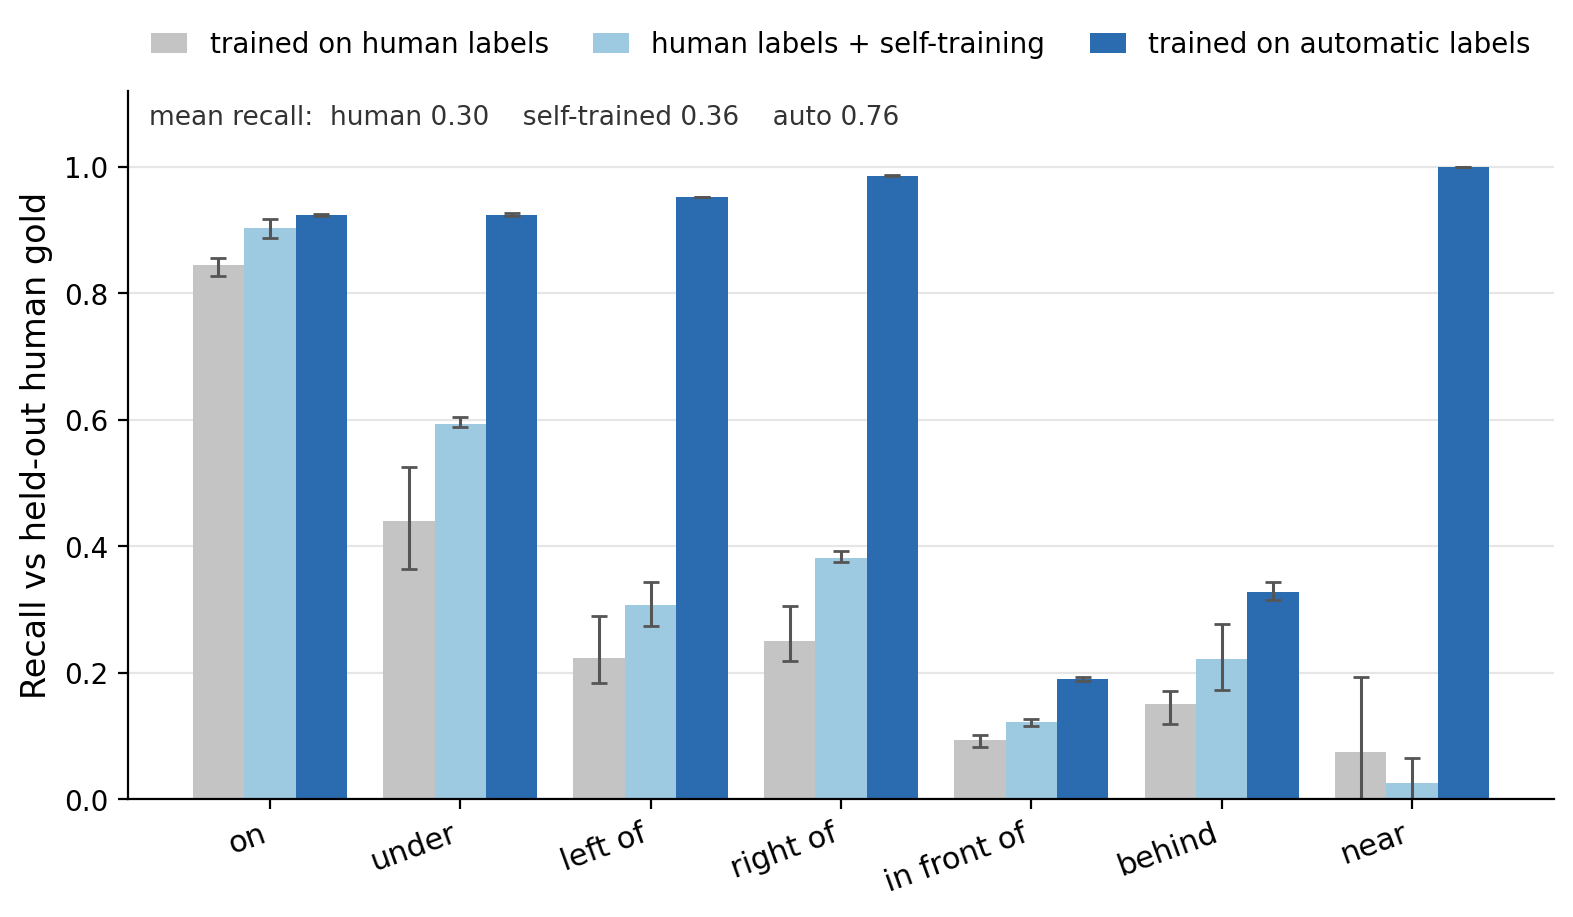
\includegraphics[width=0.95\textwidth]{figures/rq2-comparison.png}
\caption{Downstream recall against held-out human gold for the three label sources. Self-training improves on the human labels everywhere except \texttt{near}, where it falls below them.}
\label{fig:rq2-comparison}
\end{figure}

\section{Why self-training does not rescue the human labels}

The pseudo-label arm's own bookkeeping explains its ceiling precisely. Of the 60,762 training pairs, the annotators recorded just \textbf{6,026}. Filling in the rest, the teacher adds roughly \textbf{54,000 confident negative} pseudo-labels per predicate against only \textbf{36 to 67 confident positives}: a ratio of about 1,000 to 1. The teacher, trained on annotation in which most pairs carry no label, has learned above all that pairs usually have no relation, and self-training feeds that conviction back to the student as though it were evidence. What propagates is not the annotators' knowledge but their silence.

This is the failure mode \S2.4 predicted from the literature, now measured. Pseudo-labelling is well behaved when the labelled seed is a representative sample of the unlabelled pool. Here it is neither representative nor complete: the annotators labelled the pairs they found salient, so absence of a label conflates "no relation holds" with "nobody looked". A student trained on the union cannot distinguish the two, and inherits a systematic bias towards silence.

The \texttt{near} row makes the point sharply. Human-trained recall is already near-collapse at 0.08, and self-training pushes it \textit{down} to 0.03. Only three of nine annotator groups used the label at all, so the teacher's notion of "near" is both weak and idiosyncratic; its confident pseudo-labels then bury what little positive signal existed. Where the seed is defective, self-training does not merely fail to help, it can actively amplify the defect. The automatic labels reach 1.00 on the same evaluation, because the fitted threshold applies one definition to every pair rather than extrapolating three annotators' habits.

The comparison is therefore not "programmatic labels beat doing nothing", but "programmatic labels beat the standard remedy, under identical conditions, closing more than six times as much of the available gap". Active learning is not tested here because it fails for a different and simpler reason: it still buys human labels, so it lowers the bottleneck's cost without removing it, and it has no mechanism at all for the inconsistency between annotators that Chapter 4 measures.

\section{Why the automatic labels win, and two consistency checks}

The mechanism is the one this dissertation measures throughout: the human labels are \textit{sparse} (\textasciitilde{}10\% of pairs) and \textit{inconsistent} (three of nine annotators used \texttt{near}; two inverted the front/behind convention; support was often labelled in one direction only). A classifier trained on sparse, inconsistent supervision learns above all to be silent; its recall collapses exactly where human labelling was thinnest (\texttt{near} 0.08, lateral 0.22--0.25). The automatic labels are dense and rule-consistent, so the same model actually learns the geometry (near 1.00, lateral 0.95--0.99, support 0.92). This is the weak-supervision prediction (\S2.3) confirmed under controlled conditions: dense, consistent programmatic labels out-teach scarce gold labels when supervision, not model capacity, is the bottleneck.

Two checks argue the result is real rather than an artefact. First, the auto-trained model's profile almost exactly reproduces the rule layer's own held-out performance (mean 0.76; front/behind 0.19/0.33 $\approx$ the rules' held-out 0.20/0.35): the classifier \textit{distilled the annotator}, which is precisely what "the labels are learnable" means. Second, all three arms face identical conditions everywhere: the same features, the same oversampling cap, the same held-out gold including the convention-inverted annotators, which penalises every arm's front/behind equally.

\section{Honest boundaries}

The evaluation gold is itself sparse human annotation, so recall (not precision) is the reported metric, mirroring the RQ1 protocol. The human-trained model's weakness is partly a property of \textit{any} sparse supervision at this scale; with many more human labels it would improve, but producing many more human labels is exactly the bottleneck this project removes, and the self-trained arm shows the shortfall cannot simply be computed away. The front/behind rows are depressed for every arm by the held-out groups' inverted convention (Chapter 4); the comparison between sources remains fair because the penalty is shared.

One structural caveat deserves stating plainly. The classifier's features are geometric, and the automatic labels were generated by rules over closely related geometry, so the auto-trained arm's task is partly to re-learn its own generator; read alone, this chapter shows the automatic labels are \textit{learnable} and the human labels are not, rather than that automatic labels win under any featurisation. Three things keep the comparison meaningful: every arm receives the identical features, so the featurisation advantages no source; "the labels are learnable" is itself the property RQ2 asks about, since a downstream consumer must extract a consistent signal from the labels; and Chapter 6 removes the circularity entirely by repeating the comparison in a full scene-graph model with visual features, where the density and consistency effects persist in the training dynamics and the zero-shot generalisation even though the headline verdict changes.

\section{From labels to robots: where this sits in the source paper's chain}

The source paper's end goal is explicit: spatial understanding exists so that robots can plan. Their motivating example shows an LLM planner failing to remove a cube before grasping the book beneath it until SGG-derived relations are supplied, after which it "generates executable, spatially-aware plans." The paper's own evaluation of that chain stops at SGG quality: six models benchmarked on the human labels, topping out at mR@100 = 0.49 (VCTree), with every model saturating by epoch 2--6 and \texttt{near} stuck at 0.22--0.25 (\S2.2).

Each of those benchmark symptoms has a cause this dissertation measured and a remedy it built. Saturation within six epochs is what training on 9,313 sparse triplets looks like; the automatic labels provide 20$\times$ the supervision on the same images. The universal \texttt{near} failure is what training on an undefined, three-annotator label looks like; the fitted-threshold labels are perfectly learnable (this chapter's proxy reaches 1.00). And the depth predicates were being actively taught two opposite conventions by different annotators; the automatic labels apply one. The controlled experiment above is the proxy for the SGG step of the chain, and it measures the effect as large. The direct test, training the paper's own benchmark model on automatic versus human labels and comparing mR@100, is executed in Chapter 6. Three concrete predictions are registered here, before that run: later saturation, a higher plateau, and the recovery of \texttt{near}. Chapter 6 judges all three.

\section{The planner experiment: does the label source change what a robot would do?}

Section 5.6 ends with the source paper's motivating example, in which an LLM planner fails to remove a cube before grasping the book beneath it until spatial relations are supplied. That example is an assertion in the paper, illustrated on one scene. It can be run as an experiment, and this section runs it.

\textbf{Design.} Twenty-five held-out scenes were selected in which a target object has a second object physically resting on it, so any safe plan must move the occluder first. Each scene is put to an LLM planner (\texttt{gemini-flash-latest}) three times, in prompts differing only in what they state about the scene: \textbf{A} lists the objects and nothing else, \textbf{B} adds the human-annotated relationships, \textbf{C} adds the automatically computed ones. The task sentence, the object list and the instruction to give a minimal numbered plan are identical across conditions. All three conditions of a scene are answered by one model in one sitting, so no scene can be split across models by a quota interruption (\texttt{scripts/run\_planner\_llm.py}).

\textbf{Scoring.} A plan is safe if it moves the occluding object in an earlier step than the one that grasps the target. Judgements are made by published rules rather than by reading (\texttt{eval/score\_planner.py}), for two reasons: the rules never see the condition, so scoring is blind by construction, which matters when the author has a stake in the result; and a reader who disputes a verdict can inspect the rule instead of trusting a judgement. The rules were checked against a hand-read sample, which is the only thing that makes them trustworthy and which caught a real defect: models frequently open with a preamble restating the task ("To pick up box0 safely, follow these steps:"), and counting that preamble as a step made every such plan appear to grasp the target before clearing anything. Before the fix condition C scored 0.64; after it, 0.88. The figure below the fix is the correct one, and the episode is recorded because an automatic scorer is worth exactly what its agreement with careful manual reading says it is.

\textbf{Result.}

\begin{center}
\small
\begin{longtable}{lrr}
\caption{Planner experiment: whether the plan clears the occluding object before grasping the target, over 25 held-out scenes under each label source.}\\
\hline
Condition & Prompt states & Safe plans \\
\hline
\endfirsthead
\hline
Condition & Prompt states & Safe plans \\
\hline
\endhead
A & objects only & 0 / 25 \\
B & human relationships & 25 / 25 \\
C & automatic relationships & 22 / 25 \\
\hline
\end{longtable}
\end{center}

The effect of stating relations at all is total: without them the planner never clears the occluder, in twenty-five scenes out of twenty-five. Its plans are not careless, they are confidently wrong in a specific way, typically proposing to "lift the target vertically to clear all surrounding objects" while the object resting on top of it goes unmentioned. That is the paper's illustrated failure, reproduced at scale rather than asserted.

\textbf{Where the automatic labels lose, and why.} All three C failures have the same cause, and it is not a planning failure: in each, the automatic relation list did not contain the support relation. Scene 4 offered "box6 is in front of book7" and "box6 is near book7"; scene 24 offered near, in front of and to the left of. The occluder was described, accurately, in every way except the one the task depended on. In zero cases was the support relation present and ignored. The failure rate follows directly: three misses in twenty-five scenes is 12\%, against the measured support recall of 0.88 in \S4.2, so the planner result is the fidelity result showing up one level higher in the chain.

Scene 16 shows the mechanism sharply. The planner used the automatic relations it was given, cleared the four objects the prompt said were \textit{in front of} the target, and left the one resting on top of it, because that relation was never stated. It reasoned correctly from incomplete input.

\textbf{What this does not show.} Three limits. The comparison is between label sources, not planners: condition B is handed the exact fact the task tests, so B versus C measures whether each source supplies that fact, not which source produces better reasoning. It uses one model and one prompt style, so the size of the A-to-B gap is a property of this planner as much as of the labels, even though its direction is not in doubt. And no robot moved: this measures plans, not executions, so it closes the gap between labels and robot behaviour by one link rather than closing it entirely.

What it settles is the question \S5.6 could only frame. Automatic labels carry 88\% of the decision-relevant content that human labels carry on this task, against 0\% for no labels at all, and the residual gap is not a property of computed labels in general but of one predicate whose recall is already measured and whose failure mode is already diagnosed (\S4.9).

\section{Answer to RQ2}

Yes, with more than was asked. The automatic labels are not merely "good enough" to train a relation model: at this dataset's scale of human annotation, they are \textbf{substantially better training material than the human labels themselves}, because label density and consistency dominate raw human authority when supervision is sparse. The self-trained arm sharpens the claim by ruling out the cheap alternative: stretching the existing labels with the standard semi-supervised remedy recovers only 15\% of the gap, because what it propagates is the annotators' silence rather than their knowledge. This is the dissertation's core claim, that removing the human bottleneck can \textit{grow} dataset utility rather than merely approximate it, demonstrated on the dataset's own held-out annotators and against the obvious rival.

\chapter{The Direct Benchmark Test}
\input{chapter6_benchmark}

\chapter{Critical Evaluation}
\input{chapter7_critical_evaluation}

\chapter{Legal, Social, Ethical and Professional Considerations}
\input{chapter8_lsep}

\chapter{Conclusions and Future Work}

This chapter closes the dissertation. Section 9.1 states how each objective was met and what the two research questions were answered with, \S9.2 sets out the contributions and who can use them, \S9.3 states the limitations honestly and turns each into the work that would resolve it, and \S9.4 is a personal reflection on how the project was actually conducted.

\section{Summary of the dissertation}

The aim was to determine whether spatial-relationship annotation for robot-acquired images can be automated, and whether the resulting labels are good enough to replace the human ones. Five objectives carried that aim, and each is met with evidence rather than assertion.

\textbf{O1, build.} A fully-automatic pipeline annotates all 836 images in about five minutes on a 6 GB consumer GPU, with no human deciding any label, and writes the dataset's own formats byte-compatibly (Chapter 3). Verified by a load-write round trip reproducing boxes and labels with zero error.

\textbf{O2, specify and calibrate.} All seven predicates have written operational definitions with explicit thresholds, every one fitted on annotator groups 0 to 5 alone and reported on the held-out groups (Chapter 3). The \texttt{near} threshold generalises perfectly to the held-out annotator who used the label (recall 1.00), and the support rules reach held-out F1 0.87.

\textbf{O3, validate.} Per-predicate fidelity against all 8,926 human triplets, against three baselines, with eight ablations and manually audited precision (Chapter 4): mean recall 0.85, and 0.76 on annotators no threshold ever saw. Cluster-bootstrap intervals accompany every headline figure, and an independent validation study re-estimates precision with judges who have no stake in the result (\S4.13).

\textbf{O4, diagnose.} Every one of the 1,689 missed human triplets is attributed to a cause by re-checking rule conditions, so the failure analysis is exhaustive rather than illustrative. Genuine tool error accounts for roughly 7\% of misses; the remainder is calibrated abstention and measured annotator behaviour (\S4.10, \S7.2).

\textbf{O5, test downstream utility.} A controlled experiment trains the same classifier on three label sources under identical conditions (Chapter 5), and the comparison is repeated in the source paper's own benchmark framework with a shared frozen detector and three seeds per arm (Chapter 6).

\textbf{RQ1, accuracy.} Yes, with one qualification. On five of seven predicates the automatic labels match or exceed the human process (0.81 to 1.00 recall, audited precision $\approx$ 1.0), and \texttt{near} is solved outright, resolving the one predicate the source paper reports as failing for every model it benchmarked. The depth pair reaches 0.64/0.66 pooled and 0.84 once two annotator groups' inverted conventions are accounted for; where the tool commits it agrees at 0.95 to 1.00 with six of the seven same-convention annotators, the seventh being the smallest sample in the dataset. The residual limit is monocular ambiguity, which ablation A8 shows a four-times-larger depth model does not fix.

\textbf{RQ2, utility.} Yes, and by a wide margin at this dataset's annotation scale. The auto-trained classifier reaches 0.76 mean recall against held-out human gold versus 0.30 for its human-trained twin, and versus 0.36 when the human labels are stretched by self-training, the standard semi-supervised remedy. In the full benchmark the verdict is conditional and the condition is legible: over three seeds per arm the human-trained model ranks better against human test annotation (mR@100 0.326 against 0.278), the auto-trained model generalises about sixty times better to unseen relation compositions (zR@100 0.172 against 0.003, with disjoint per-seed ranges), and the human advantage is concentrated entirely on the two test annotators carrying measured labelling defects, disappearing against the only one without (0.308 against 0.307).

The single sentence the evidence supports: \textbf{automatic labels are the better supervision wherever ground truth means geometry; human labels remain better wherever ground truth means human annotation practice.} Robot planning needs the former.

\section{Research contributions}

\textbf{For the source dataset and its authors.} An annotator that labels the existing images 20 times more densely in five minutes, in the dataset's own formats, and the written operational definitions the annotation process never had. The fitted \texttt{near} threshold is a direct answer to the future-work request in Wang et al. (2025) for "spatial thresholds for near". Two annotation defects are quantified for the first time: an inverted front/behind convention in two of nine annotator groups, and \texttt{near} used by only three groups with fourfold variation in exhaustiveness.

\textbf{For work on scene-graph benchmarks.} Evidence that ranked recall against sparse, guideline-free annotation partly measures agreement with annotator habits rather than spatial correctness. The evidence is a dissociation: the model that ranks better memorises which pairs annotators record, and the model that generalises to unseen compositions is the one trained on consistent computed labels. The per-annotator decomposition localises the effect precisely, and the seed replication shows which parts of it survive training variance.

\textbf{For weak supervision.} A controlled three-way comparison, on the same features, model, split and seeds, showing that programmatic labels out-teach both scarce human labels and the standard remedy for scarce human labels. The mechanism is measured rather than inferred: self-training contributes roughly a thousand confident negative pseudo-labels for every positive one, propagating the annotators' silence rather than their judgement.

\textbf{Methodologically.} Calibration held out by \textit{annotator} rather than by image; a sparse-gold evaluation protocol that pairs recall with audited precision; exhaustive loss attribution; a way to estimate what annotators would score against one another when they never labelled the same images, by using a deterministic annotator as a fixed common reference (\S4.6); and a reliability check that needs no labels at all, obtained by recovering the fact that an image dataset was cut from a continuous capture and asking whether its labels survive the camera moving (\S4.14). The last of these is the one most likely to transfer. Many robotics datasets are sequences presented as image sets, and wherever that is true, a predicate's agreement with itself across viewpoints separates a rule that is wrong from a rule that is merely uncertain, which is a distinction sparse human annotation cannot draw.

\section{Limitations, and future research and development}

Each limitation below is stated with the specific experiment that would settle it, because that is more useful than an apology.

\textbf{The chain stops short of the robot.} The strongest evidence reaches label quality and model quality; no experiment in this dissertation shows a robot completing more tasks. The instrument exists: 75 prompts across 25 held-out scenes in three conditions (no relations, human relations, automatic relations), with a blind scoring sheet, built and ready to run. This is the single most valuable next experiment, and it is the one that would convert a supported inference into a demonstration.

\textbf{Precision estimates remain partly author-verdicted.} The independent validation study (\S4.13) is deployed and collecting, with coverage stratified so the audit-overlap items reach several raters first. Until it completes, the audited precision figures carry the author's own judgement, conservatively applied and published for checking.

\textbf{One domain, one camera, six object classes.} The fitted constants are dataset-specific by design; what transfers is the calibration procedure. The only out-of-domain evidence is qualitative (\S4.12), where unretuned thresholds behaved correctly on stock video containing objects outside the six classes. A labelled cross-domain sample of a few dozen images would turn that into a measurement, and it is cheap enough that a replication should simply include one.

\textbf{Front/behind is bounded by monocular ambiguity.} Two objects at similar camera distance cannot be ordered from one image, and a larger depth model does not help (A8). The routes out are additional evidence rather than better models: stereo or RGB-D capture, multi-frame structure, or wider surface detection to extend the ground-plane guard, the last of which was built, measured and declined on this dataset (\S4.9.4).

\textbf{Detection bounds full automation.} With a zero-shot detector the end-to-end recall is 0.38, while the relation layer conditional on detection scores 0.85. The gap is detection, not relations, and the source paper's own trained detector (0.93 mAP@50) would close most of it. That check needs only the released weights.

\textbf{Scale is demonstrated without ground truth.} The supervising group supplied the full 2,650-frame capture the released images were cut from, and the pipeline was run over the 1,766 frames nobody has annotated: 562 keyframes after content-adaptive selection, 31 minutes, 185,242 triplets, a predicate distribution 0.032 in total variation from the annotated portion (\S4.15). Capacity and stability on unfamiliar input are therefore measured rather than argued. Correctness on that portion is not, and cannot be without labels; \S4.14's viewpoint-consistency check substitutes self-agreement for truth and should be read as the weaker thing it is. The experiment that would close this is a modest labelled sample from the unannotated frames, a few hundred triplets, which is an afternoon of annotation rather than a research programme.

\textbf{The capture is stereo, and only one eye was used.} The supplied folder is named \texttt{rightimg}, which implies a left counterpart held by the supervising group. True stereo would attack the front/behind bound directly, supplying disparity where this project has only monocular relative depth, and would do so at every frame rather than requiring the robot to move. Multi-frame structure is the weaker fallback if no left channel survives: measured on this sequence, consecutive frames carry 0.08 px of motion, far too little for parallax, with usable baselines appearing only around 20 to 40 frames apart. That route also changes the method's premise, since depth recovered from twenty frames of robot walking is not available to a single-image annotator, so it belongs to a validation instrument rather than to the pipeline.

\section{Personal reflections}

The most useful thing this project taught me was to distrust a number until I know how it was produced.

That lesson arrived early and painfully. My first depth-based results were poor, and the unit tests all passed. The cause was that the dataset's images are stored rotated 180 degrees behind an EXIF flag, so every mask and depth value was being read from an upside-down image while the boxes stayed upright. No automated check could have caught it, because every component was behaving exactly as written. I found it by rendering an image with its boxes drawn on and looking at it. Since then I have rendered and inspected samples after every significant change, and it has caught things twice more.

The second lesson was that "agreement with the humans" is not one target. I began by treating the human labels as ground truth and my disagreements as errors. Measuring them properly showed that three of nine annotator groups used \texttt{near} at all, that two labelled front and behind in opposite directions, and that some labelled support in only one direction. That reframed the project: the interesting question stopped being "how close can I get to the humans" and became "what exactly do the humans mean, and where do they disagree with each other". Almost every later design decision, including calibrating on some annotators and validating on others, follows from that shift.

The third lesson was about my own claims, and it is the one I would most like to have learned sooner. Reading a single benchmark run, I reported that my labels won against the one test annotator with clean conventions. The margin was 0.011 on 73 images. When I later retrained both arms at two more seeds, the arms turned out to be tied, and I withdrew the claim (\S6.3.1). I had been careful about this in one place, fitting thresholds on some annotators and validating on others, and careless about it in another, treating one training run as a result. The discipline was not new to me; I simply had not applied it to model training variance. Recording the retraction in the chapter rather than quietly deleting it felt uncomfortable and is, I think, the right thing to have done.

What I would do differently, given the time again, is front-load the experiments that answer the question the project actually asks. I spent considerable effort proving that the labels are correct and that they train models well, and comparatively little on whether they help a robot decide what to do, which is the entire motivation. The planner experiment should have run in week five rather than sitting built and unrun at the end. I would also have arranged for two people to annotate the same fifty images in week two: that one afternoon would have produced the inter-annotator agreement figure that the whole "comparable to human quality" claim needs, and which I ended up estimating indirectly instead.

Technically, the thing I am most pleased with is not the accuracy figure but the two refinements I built, measured and then declined. Both were plausible, both took real work, and the data said neither helped. Reporting them as null results rather than dropping them was the point at which the project started feeling like research rather than engineering.

%==================== References ====================
\chapter*{References}
\addcontentsline{toc}{chapter}{References}
\begin{description}[leftmargin=2em, labelindent=0em]
\item[] Ahn, M. et al. (2022) 'Do as I can, not as I say: grounding language in robotic affordances', \textit{Proceedings of the 6th Conference on Robot Learning (CoRL)}. Available at: https://arxiv.org/abs/2204.01691
\item[] Armeni, I., He, Z.-Y., Gwak, J., Zamir, A.R., Fischer, M., Malik, J. and Savarese, S. (2019) '3D scene graph: a structure for unified semantics, 3D space, and camera', \textit{Proceedings of the IEEE/CVF International Conference on Computer Vision (ICCV)}.
\item[] Artstein, R. and Poesio, M. (2008) 'Inter-coder agreement for computational linguistics', \textit{Computational Linguistics}, 34(4), pp. 555--596.
\item[] Azevedo, A. and Santos, M.F. (2008) 'KDD, SEMMA and CRISP-DM: a parallel overview', \textit{Proceedings of the IADIS European Conference on Data Mining}, pp. 182--185.
\item[] BCS (2022) \textit{BCS Code of Conduct}. Swindon: BCS, The Chartered Institute for IT. Available at: https://www.bcs.org/membership-and-registrations/become-a-member/bcs-code-of-conduct/
\item[] Chang, X., Ren, P., Xu, P., Li, Z., Chen, X. and Hauptmann, A. (2023) 'A comprehensive survey of scene graphs: generation and application', \textit{IEEE Transactions on Pattern Analysis and Machine Intelligence}, 45(1), pp. 1-26.
\item[] Chen, B., Xu, Z., Kirmani, S., Ichter, B., Driess, D., Florence, P., Sadigh, D., Guibas, L. and Xia, F. (2024) 'SpatialVLM: endowing vision-language models with spatial reasoning capabilities', \textit{Proceedings of the IEEE/CVF Conference on Computer Vision and Pattern Recognition (CVPR)}. Available at: https://arxiv.org/abs/2401.12168
\item[] Cheng, A.-C. et al. (2024) 'SpatialRGPT: grounded spatial reasoning in vision-language models', \textit{Advances in Neural Information Processing Systems (NeurIPS)}. Available at: https://arxiv.org/abs/2406.01584
\item[] Cohen, J. (1960) 'A coefficient of agreement for nominal scales', \textit{Educational and Psychological Measurement}, 20(1), pp. 37--46.
\item[] \textit{Computer Misuse Act 1990}, c. 18. Available at: https://www.legislation.gov.uk/ukpga/1990/18/contents
\item[] \textit{Data Protection Act 2018}, c. 12. Available at: https://www.legislation.gov.uk/ukpga/2018/12/contents
\item[] Fayyad, U., Piatetsky-Shapiro, G. and Smyth, P. (1996) 'From data mining to knowledge discovery in databases', \textit{AI Magazine}, 17(3), pp. 37--54.
\item[] Goyal, A., Yang, K., Yang, D. and Deng, J. (2020) 'Rel3D: a minimally contextualized benchmark for grounding spatial relations in 3D', \textit{Advances in Neural Information Processing Systems (NeurIPS)}.
\item[] Gu, Q. et al. (2024) 'ConceptGraphs: open-vocabulary 3D scene graphs for perception and planning', \textit{Proceedings of the IEEE International Conference on Robotics and Automation (ICRA)}.
\item[] Hughes, N., Chang, Y. and Carlone, L. (2022) 'Hydra: a real-time spatial perception system for 3D scene graph construction and optimization', \textit{Robotics: Science and Systems (RSS)}.
\item[] Johnson, J., Hariharan, B., van der Maaten, L., Fei-Fei, L., Zitnick, C.L. and Girshick, R. (2017) 'CLEVR: a diagnostic dataset for compositional language and elementary visual reasoning', \textit{Proceedings of the IEEE Conference on Computer Vision and Pattern Recognition (CVPR)}.
\item[] Krishna, R. et al. (2017) 'Visual Genome: connecting language and vision using crowdsourced dense image annotations', \textit{International Journal of Computer Vision}, 123(1), pp. 32--73.
\item[] Landau, B. and Jackendoff, R. (1993) '"What" and "where" in spatial language and spatial cognition', \textit{Behavioral and Brain Sciences}, 16(2), pp. 217-238.
\item[] Lee, D.-H. (2013) 'Pseudo-label: the simple and efficient semi-supervised learning method for deep neural networks', \textit{ICML Workshop on Challenges in Representation Learning}.
\item[] Liu, S. et al. (2024) 'Grounding DINO: marrying DINO with grounded pre-training for open-set object detection', \textit{Proceedings of the European Conference on Computer Vision (ECCV)}. Available at: https://arxiv.org/abs/2303.05499
\item[] Lu, C., Krishna, R., Bernstein, M. and Fei-Fei, L. (2016) 'Visual relationship detection with language priors', \textit{Proceedings of the European Conference on Computer Vision (ECCV)}.
\item[] Neau, M. and Falomir, Z. (2026) 'REACT++: efficient cross-attention for real-time scene graph generation'. arXiv preprint. Available at: https://arxiv.org/abs/2603.06386
\item[] Northcutt, C.G., Athalye, A. and Mueller, J. (2021) 'Pervasive label errors in test sets destabilize machine learning benchmarks', \textit{Advances in Neural Information Processing Systems (NeurIPS), Datasets and Benchmarks Track}.
\item[] Radford, A. et al. (2021) 'Learning transferable visual models from natural language supervision', \textit{Proceedings of the 38th International Conference on Machine Learning (ICML)}, PMLR 139, pp. 8748--8763.
\item[] Ratner, A., Bach, S.H., Ehrenberg, H., Fries, J., Wu, S. and Ré, C. (2017) 'Snorkel: rapid training data creation with weak supervision', \textit{Proceedings of the VLDB Endowment}, 11(3), pp. 269--282.
\item[] Ravi, N. et al. (2024) 'SAM 2: segment anything in images and videos'. arXiv preprint. Available at: https://arxiv.org/abs/2408.00714
\item[] Remyx AI (2024) \textit{VQASynth} [computer program]. Available at: https://github.com/remyxai/VQASynth
\item[] Settles, B. (2009) \textit{Active learning literature survey}. Computer Sciences Technical Report 1648, University of Wisconsin--Madison.
\item[] Song, C.H., Blukis, V., Tremblay, J., Tyree, S., Su, Y. and Birchfield, S. (2025) 'RoboSpatial: teaching spatial understanding to 2D and 3D vision-language models for robotics', \textit{Proceedings of the IEEE/CVF Conference on Computer Vision and Pattern Recognition (CVPR)}, oral presentation. Available at: https://arxiv.org/abs/2411.16537
\item[] Tang, K., Zhang, H., Wu, B., Luo, W. and Liu, W. (2019) 'Learning to compose dynamic tree structures for visual contexts', \textit{Proceedings of the IEEE/CVF Conference on Computer Vision and Pattern Recognition (CVPR)}.
\item[] Tang, K., Niu, Y., Huang, J., Shi, J. and Zhang, H. (2020) 'Unbiased scene graph generation from biased training', \textit{Proceedings of the IEEE/CVF Conference on Computer Vision and Pattern Recognition (CVPR)}.
\item[] Uma, A.N., Fornaciari, T., Hovy, D., Paun, S., Plank, B. and Poesio, M. (2021) 'Learning from disagreement: a survey', \textit{Journal of Artificial Intelligence Research}, 72, pp. 1385--1470. doi:10.1613/jair.1.12752
\item[] van Engelen, J.E. and Hoos, H.H. (2020) 'A survey on semi-supervised learning', \textit{Machine Learning}, 109(2), pp. 373--440.
\item[] Wang, A. et al. (2024) 'YOLOv10: real-time end-to-end object detection', \textit{Advances in Neural Information Processing Systems (NeurIPS)}. Available at: https://arxiv.org/abs/2405.14458
\item[] Wang, F., Mei, J. and Yuille, A. (2024) 'SCLIP: rethinking self-attention for dense vision-language inference', \textit{Proceedings of the European Conference on Computer Vision (ECCV)}. Available at: https://arxiv.org/abs/2312.01597
\item[] Wang, P., Pham, M.H., Guo, Z. and Zhou, W. (2025) 'A spatial relationship aware dataset for robotics', \textit{Proceedings of the 33rd ACM International Conference on Multimedia (MM '25)}. doi:10.1145/3746027.3758293
\item[] Wirth, R. and Hipp, J. (2000) 'CRISP-DM: towards a standard process model for data mining', \textit{Proceedings of the 4th International Conference on the Practical Applications of Knowledge Discovery and Data Mining}, pp. 29--39.
\item[] Xie, Q., Luong, M.-T., Hovy, E. and Le, Q.V. (2020) 'Self-training with Noisy Student improves ImageNet classification', \textit{Proceedings of the IEEE/CVF Conference on Computer Vision and Pattern Recognition (CVPR)}.
\item[] Yang, J., Ang, Y.Z., Guo, Z., Zhou, K., Zhang, W. and Liu, Z. (2022) 'Panoptic scene graph generation', \textit{Proceedings of the European Conference on Computer Vision (ECCV)}.
\item[] Yang, K., Russakovsky, O. and Deng, J. (2019) 'SpatialSense: an adversarially crowdsourced benchmark for spatial relation recognition', \textit{Proceedings of the IEEE/CVF International Conference on Computer Vision (ICCV)}.
\item[] Yang, L. et al. (2024) 'Depth Anything V2', \textit{Advances in Neural Information Processing Systems (NeurIPS)}. Available at: https://arxiv.org/abs/2406.09414
\item[] Ye, J. et al. (2025) 'PrimitiveAnything: human-crafted 3D primitive assembly generation with auto-regressive transformer', \textit{ACM SIGGRAPH 2025 Conference Papers}. Available at: https://arxiv.org/abs/2505.04622
\item[] Zellers, R., Yatskar, M., Thomson, S. and Choi, Y. (2018) 'Neural Motifs: scene graph parsing with global context', \textit{Proceedings of the IEEE/CVF Conference on Computer Vision and Pattern Recognition (CVPR)}.
\item[] Zhang, W. et al. (2025) 'Open3D-VQA: a benchmark for embodied spatial concept reasoning with multimodal large language model in open space', \textit{Proceedings of the 33rd ACM International Conference on Multimedia (MM '25)}. doi:10.1145/3746027.3758219
\end{description}

%==================== Appendices ====================
% Named as the template's contents page requires: Appendix A is the ethics
% record, later appendices are supplementary material.
\appendix
\renewcommand{\chaptertitlename}{Appendix}
\chapter{Ethical Approval}


This project performs secondary analysis of an existing, published research dataset (Wang et al., 2025; released under CC-BY 4.0), collected by the project supervisor's research group using a Boston Dynamics Spot robot. No new personal data was collected for the annotation study. Scene images in the dataset contain identifiable people; all figures reproduced in this dissertation blur faces, and the dataset is used strictly as released.

A second body of data is used in \S4.14 and \S9.3: the complete 2,650-frame capture from which the released images were cut, supplied directly by the supervising group. Frames 000000--000883 are the released dataset itself, verified by exact pixel match; the remaining 1,766 frames carry no annotation and are \textbf{not} covered by the CC-BY release. They are used here only to measure the pipeline's behaviour on unlabelled input, they are not redistributed with this work, and no figure reproduces a frame from them without the supervisor's specific agreement. They show the same laboratory and the same people as the released portion, and the face-anonymisation rule above applies to them unchanged.

The independent validation of the automatic labels (Chapter 4) collects anonymous true/false judgements from adult volunteers through a purpose-built web quiz. No names, email addresses, IP addresses or any other personal data are recorded; each browser receives a random identifier used only to spread item coverage and remove duplicate answers. Participation is voluntary, takes about three minutes, and can be abandoned at any point; an information panel on the first screen states the purpose, the data collected, and a contact address. Faces in all quiz images are pixelated before publication, and items where anonymisation would obscure the object under judgement were removed rather than shown. The collection is covered by the University's ethics self-assessment process, completed and submitted on 19 July 2026. Because the study collects no personal data, involves no vulnerable groups and carries no foreseeable risk beyond that of everyday life, it falls within the self-assessment route rather than requiring full committee review.

\textit{The completed self-assessment form is attached at the end of this appendix.}

\textbf{Demonstration footage.} The two video clips in \S4.12 are royalty-free stock footage from Pexels, used under the Pexels licence (free use, no attribution required): clip 1 (desk scene, moving camera) https://www.pexels.com/video/6558513/ and clip 2 (overhead desk, moving hands) https://www.pexels.com/video/a-person-working-with-pictures-and-photos-taken-using-a-modern-camera-3250234/.


\chapter{Reproducibility}


Environment: Windows 11, Python 3.11.9 (virtual environment), PyTorch 2.5.1 (CUDA 12.1), single NVIDIA RTX 2060 (6 GB). All thresholds, seeds and model identifiers are pinned in \texttt{configs/default.yaml}.

Key commands:

\begin{itemize}
\item \texttt{python scripts/run\_annotator.py}: annotate the full dataset (GPU, \textasciitilde{}5 min)
\item \texttt{python scripts/reannotate\_from\_cache.py}: re-evaluate rule changes offline
from the geometry cache (\textasciitilde{}20 s, no GPU)
\item \texttt{python eval/fit\_near.py}: fit and report the \texttt{near} threshold
\item \texttt{python eval/fidelity.py}: the RQ1 battery $\rightarrow$ \texttt{outputs/}
\item \texttt{python eval/uncertainty.py --iters 2000}: cluster-bootstrap intervals for
every headline recall $\rightarrow$ \texttt{outputs/tables/uncertainty.md}
\item \texttt{python eval/annotator\_agreement.py}: annotator heterogeneity and the
estimated human-human agreement bounds $\rightarrow$ \texttt{outputs/tables/annotator\_agreement.md}
\item \texttt{python eval/ablations.py}: ablations A1--A7 $\rightarrow$ \texttt{outputs/tables/ablations.md}
\item \texttt{python eval/depth\_ablation.py}: the A8 depth-model comparison
\item \texttt{python eval/parallax\_ablation.py --method triangulate --gap 10}: the
A9 multi-frame depth comparison; needs the raw capture (Appendix D.6) $\rightarrow$ \texttt{outputs/parallax\_ablation.json}
\item \texttt{python eval/seed\_stats.py}: aggregates the benchmark arms across seeds $\rightarrow$
\texttt{outputs/tables/seed\_replication.md}
\item \texttt{python eval/keyframe\_propagation.py --sweep 5,10,20,30}: content-adaptive
frame selection and the viewpoint-stability measurement of \S4.14 $\rightarrow$ \texttt{outputs/keyframe\_propagation.json}
\item \texttt{python eval/video\_stability.py}: the persistence and Jaccard figures of
\S4.12, derived from the recorded per-frame files $\rightarrow$ \texttt{outputs/video\_stability.json}
\item \texttt{python eval/extension\_scale.py}: throughput, density and predicate
distribution on the unannotated capture (\S4.15) $\rightarrow$ \texttt{outputs/extension\_scale.json}
\item \texttt{python scripts/run\_vlm\_pilot.py --make} then \texttt{python scripts/run\_vlm\_pilot.py}
then \texttt{python eval/score\_vlm\_pilot.py}: the \S4.16 vision-language comparison (30 numbered-box images, RQ1 battery, self-consistency diagnostics) $\rightarrow$ \texttt{outputs/vlm\_pilot/}. The second model is the same three commands with \texttt{--model} and its own \texttt{--replies} file, then \texttt{python eval/compare\_vlm\_models.py} $\rightarrow$ \texttt{outputs/tables/vlm\_models.md}. Reasoning models need \texttt{--max-output-tokens} above the 8192 default, because they spend most of the budget deliberating and a truncated reply is indistinguishable from a malformed one. \texttt{python scripts/vlm\_manual\_check.py} then writes a pack that lets the comparison be redone by hand in a browser: the image the model saw, the prompt verbatim, and the human, pipeline and model answers side by side, so the scoring script can be checked without running it.
\item \texttt{python scripts/run\_planner\_llm.py} then \texttt{python eval/score\_planner.py}:
the \S5.7 planner experiment (75 prompts over 25 scenes in three conditions) and its rule-based blind scoring $\rightarrow$ \texttt{outputs/planner/}, \texttt{outputs/planner\_scores.json}. Both runner and scorer take \texttt{--replies}, which is how the second planner was run into \texttt{replies\_pro.jsonl} and scored into \texttt{planner\_scores\_pro.json} without touching the first. Add \texttt{--sample N} to print plans with their verdicts for manual checking.
\item \texttt{python eval/downstream.py --seeds 42,43,44}: the RQ2 experiment, all three
label sources (human, self-trained, automatic)
\item \texttt{python analysis/score\_votes.py votes.csv}: scores the independent
validation study (crowd precision, author-bias kappa, rater reliability); lives with the study's own repository
\item \texttt{python scripts/make\_figures.py}: regenerate all figures from cached results
\item \texttt{pytest -q}: unit and invariant tests
\end{itemize}

The Chapter 6 experiment is reproducible from \texttt{scripts/kaggle/}: the dataset converters (\texttt{export\_sgg\_benchmark.py}, \texttt{export\_yolo\_det.py}), the adapted REACT++ configuration, the run recipes (\texttt{README.md}, \texttt{notebook\_cells.md}, and \texttt{seed\_replication.ipynb} for the seed replication), and the executed evaluation notebook with its outputs (\texttt{eval\_notebook.ipynb}), which is the recorded provenance of every number in Chapter 6's tables. Training logs and parsed results: \texttt{outputs/sgg\_benchmark/}.

\subsection{Full reproduction walk-through}

\textbf{1. Environment.} Either build the container (\texttt{docker build -t spatial-annotator .}) or create a Python 3.11/3.12 venv and follow the three numbered notes at the top of \texttt{requirements.txt}. The known pitfall is documented in those notes: installing SAM2 can silently replace CUDA torch with a CPU wheel, fixed by reinstalling torch with \texttt{--no-deps --force-reinstall} from the cu121 index. Either way, verify with \texttt{python scripts/smoke\_test.py --image assets/sample.jpg}, which loads SAM2 and Depth Anything and reports CUDA availability and peak memory (\textasciitilde{}0.65 GB).

The \texttt{Dockerfile} at the repository root pins Python 3.11, torch 2.5.1 + cu121 and installs SAM2 from GitHub, applying that same fix in the build itself, and a \texttt{.dockerignore} holds the build context to the 94 source files that belong in an image, keeping the caches, the dataset and the credentials file out of it. Both moving parts are pinned rather than tracked: the base image by digest, since a tag can be re-pointed upstream, and SAM2, which has no PyPI release, to commit \texttt{2b90b9f5}, since installing from a bare repository URL fetches whatever \texttt{main} happens to be on the day of the build.

The build has been run rather than merely written, and its log is kept at \texttt{outputs/docker/build\_summary.txt}: the base image in 193 s, system packages in 31 s, and the Python dependencies, including SAM2 and the forced CUDA torch reinstall, in 328 s. The final stage runs the project's test suite \textit{inside the container} and reports \textbf{66 passed} followed by a successful import of the rule layer, so an environment that cannot import the rule layer cannot produce an image at all.

The resulting image, 7.02 GB over eleven layers, was then checked as an artefact rather than trusted on the strength of its log, because the machine that built it ran out of disk during the export stage and a partly written layer is not always an obvious failure. Reading every one of the 84,972 files in the image returned no errors, so no layer is truncated. Inside the finished image the test suite reports \textbf{66 passed} a second time, torch resolves to \texttt{2.5.1+cu121} rather than the CPU wheel the pitfall above produces, and \texttt{pip check} is clean apart from a platform-metadata note on \texttt{ninja}, a build-time dependency of SAM2. The 60 Python and YAML files under \texttt{src/}, \texttt{eval/}, \texttt{tests/}, \texttt{configs/} and \texttt{scripts/} are hash-identical to the working tree, \texttt{/app} is 2.0 MB, and the dataset, the caches and the credentials file are absent, \texttt{.env.example} being the only environment file shipped.

Given a \texttt{--gpus all} flag the container also sees the card: CUDA reports available, the RTX 2060 is enumerated, and a matrix product executes on the device, so the GPU commands in the \texttt{Dockerfile} header are reachable rather than aspirational.

The end-to-end check is the one that matters for reproducibility. Mounting the dataset and the geometry cache read-only into the container and running \texttt{scripts/reannotate\_from\_cache.py} re-annotated all 836 images and produced a \texttt{pairs.csv} byte-identical to the one in this repository, 84,881 rows sharing its SHA-256, together with the same 2,508 annotation files. The container therefore does not merely install; it reproduces the annotations this dissertation reports, exactly.

\textbf{2. Data.} Clone the released dataset (CC-BY 4.0) and point \texttt{dataset.root} in \texttt{configs/default.yaml} at it. The loader expects the release's own layout (\texttt{img\_data/group\_N/*.jpg} plus the annotation JSONs) and corrects the images' 180$^{\circ}$ EXIF orientation itself; nothing is preprocessed on disk.

\textbf{3. One GPU pass, then everything is offline.} \texttt{python scripts/run\_annotator.py} (\textasciitilde{}5 min on the RTX 2060) writes the annotations in all three native formats plus the geometry, contact and depth caches under \texttt{outputs/}, and \texttt{outputs/pairs.csv}. Every experiment below runs from those caches on CPU:

\begin{center}
\small
\begin{longtable}{lrr}
\caption{Commands reproducing every experiment from the cached geometry, with run times.}\\
\hline
command & produces & time \\
\hline
\endfirsthead
\hline
command & produces & time \\
\hline
\endhead
\texttt{pytest -q} & 66 unit and invariant tests & <1 min \\
\texttt{python scripts/reannotate\_from\_cache.py} & re-runs the rules after any threshold change & \textasciitilde{}20 s \\
\texttt{python eval/fit\_near.py} & the near-threshold protocol, \texttt{near\_fit.json} & \textasciitilde{}1 min \\
\texttt{python eval/fidelity.py} & the RQ1 battery, \texttt{fidelity\_report.json} & \textasciitilde{}2 min \\
\texttt{python eval/uncertainty.py --iters 2000} & cluster-bootstrap CIs & \textasciitilde{}2 min \\
\texttt{python eval/annotator\_agreement.py} & heterogeneity + Fréchet bounds & <1 min \\
\texttt{python eval/keyframe\_propagation.py --sweep 5,10,20,30} & \S4.14 segmentation, stability, propagation cost & \textasciitilde{}3 min \\
\texttt{python eval/ablations.py} & A1--A6 sweeps & \textasciitilde{}10 min \\
\texttt{python eval/depth\_ablation.py} & A8 (needs the \texttt{outputs\_base} pass) & <1 min \\
\texttt{python eval/downstream.py --seeds 42,43,44} & RQ2, three arms & \textasciitilde{}4 h CPU \\
\texttt{python scripts/make\_figures.py} & every figure & \textasciitilde{}1 min \\
\hline
\end{longtable}
\end{center}

The two GPU extras: \texttt{python scripts/run\_sgdet.py --threshold 0.25} for the deployment-mode pass (\textasciitilde{}47 min) and \texttt{python scripts/run\_annotator.py --config configs/depth\_base.yaml --out outputs\_base} for A8's Base-model pass (\textasciitilde{}7 min).

\textbf{4. The benchmark (Chapter 6)} runs on Kaggle rather than locally (REACT++ training needs more than 6 GB): upload \texttt{datasets/spatial\_sgg\_upload.zip} (built by \texttt{scripts/export\_sgg\_benchmark.py} and \texttt{scripts/export\_yolo\_det.py}), then commit the notebooks in \texttt{scripts/kaggle/} in order (the training run in \texttt{notebook\_cells.md}, the seed replication in \texttt{seed\_replication.ipynb}, and the re-evaluation in \texttt{reeval\_seeds\_and\_groups.ipynb}) on a T4 x2 accelerator. Download each committed version's outputs into \texttt{outputs/sgg\_benchmark/} and run \texttt{python eval/seed\_stats.py}. The two framework traps are documented in the notebooks themselves: class index 0 is reserved (patched idempotently in a cell), and \texttt{--eval-only} is silently a no-op with this config, so evaluation calls \texttt{inference()} directly.

\textbf{5. The validation study} lives in its own public repository (\texttt{robot-factcheck}): \texttt{tools/build\_validation\_set.py} regenerates the claim set and site images from this repository's caches, and \texttt{analysis/score\_votes.py} scores the exported votes sheet. The private answer key never enters the public repository.

Every reported number traces to one of the JSON/markdown artefacts these commands write; no figure or table in this dissertation is produced by hand.


\chapter{Predicate specification}


The complete geometric specification of the seven predicates (definitions, thresholds, worked examples, and the correction and flagging rules) is maintained in the repository at \texttt{docs/predicate\_spec.md} and is reproduced in the submitted version of this document.


\chapter{Ablation derivations}


Chapter 4 (\S4.9) summarises the nine ablations and their verdicts. This appendix gives the derivations: how each shipped parameter was calibrated on the training annotator groups, what the held-out groups then reported, and what the audits of the affected predictions found. The two declined refinements are included in full, because a negative result is only useful if the reader can see what was actually tried.

\subsection{D.1 The support depth co-location gate (ablation A1)}

The audit's support-precision failure has a geometric cause: on a floor plane, "farther" projects as "higher in the image", so a behind-pair produces the same 2D box signature as a stacked pair. The repair is a depth co-location condition on \texttt{on}/\texttt{under} (truly stacked objects share a camera distance), an instance of the reject-the-geometrically-impossible correction principle adapted from Open3D-VQA (Zhang et al., 2025; \S2.5), calibrated on the train groups (\texttt{on\_depth\_eps} = 0.06) and validated held-out (ablation A1): support F1 on never-seen annotators rises 0.58 $\rightarrow$ 0.71. Downstream effects on the headline table: support recall -2/-3 points, \texttt{on} restricted precision 0.57 $\rightarrow$ 0.73, 44\% fewer support emissions (of the 26 audited false positives, the gate removes 12 while keeping all 4 true positives), and, because fewer false contacts suppress fewer proximity labels, \texttt{near} recall rises 0.87 $\rightarrow$ 0.95 (held-out 1.00). Mean recall is unchanged at 0.79 with a substantially more trustworthy label set. The residual false fires are same-depth cluster neighbours, which depth cannot separate by construction; they are addressed next.

\subsection{D.2 The mask-contact rule (ablation A5)}

The support signature that boxes cannot see, masks can: A rests on B iff the pixels directly below A's mask-bottom boundary belong to B (\texttt{src/contact.py}), which captures both stacking and the containment case, and rejects side-by-side neighbours. Calibrated on the train groups (\texttt{on\_contact\_min} = 0.60; the train-F1 plateau is flat from 0.60--0.80, so the choice is uncritical), ablation A5: support F1 on held-out annotators rises again, 0.71 $\rightarrow$ \textbf{0.87}, with \texttt{on} recall 0.82 $\rightarrow$ 0.88 and restricted precision 0.73 $\rightarrow$ 0.88 simultaneously, the rare change that improves both error directions at once, exactly as the failure gallery and audit predicted. Knock-on: \texttt{near} recall reaches \textbf{0.997 pooled (715/717; the two residual misses are contact-boundary cases, \S4.10) and 1.00 held-out} as the last contact-boundary suppressions disappear; headline mean recall 0.79 $\rightarrow$ \textbf{0.81}. The A4 sweep confirms the fitted threshold sits exactly at the recall plateau's knee: recall is flat from T = 1.372 upward while emissions keep growing, so the fitted value is the least-permissive point achieving maximal agreement. A 30-sample re-audit of the new support extras confirms the precision claim independently: extras correct rise from 1/15 and 3/15 (box rule) to \textbf{11/15 and 12/15}, an estimated true support precision of \textasciitilde{}0.27 $\rightarrow$ \textasciitilde{}0.9. The seven remaining wrong/uncertain extras have structure: a person \textit{holding} a remote fires contact (holding $\neq$ resting), one occluded bottle-behind-bottle pair, and three distant clusters too small to verdict confidently. The person-holding mode is closed by a \textbf{class-aware guard}: annotators never label person-support (0 of 2,466 gold support triplets involve a person on either side), so \texttt{on}/\texttt{under} are simply not evaluated for that class, removing \textasciitilde{}130 false emissions at no recall cost, since the person side carried no gold to recover.

\subsection{D.3 The ground-plane fallback (ablation A7)}

The depth abstention band was the single largest miss cause, and most of it is resolvable without depth at all: two objects standing on the same floor are depth-ordered by pure projection. The nearer object's box bottom sits lower in the image, a pixel-precise cue exactly where relative depth is noisiest. The shipped rule fires only where the depth rule abstained, only when \textit{neither} object rests on another object by the tool's own contact evidence (an elevated object's box bottom locates its support, not itself), and only outside a small bottom-edge band (\texttt{plane\_band} = 0.005, calibrated on the train groups; ablation A7). On the train groups the fallback adds 386 committed directions at 0.91 agreement; on held-out group 7 it adds 54 and \textbf{every one agrees with the annotator}. Effect on the headline: front/behind recall 0.52/0.55 $\rightarrow$ \textbf{0.64/0.66} (aligned overall 0.67 $\rightarrow$ \textbf{0.84}), mean recall 0.81 $\rightarrow$ \textbf{0.85}, and the depth-ambiguous flag rate falls 29.5\% $\rightarrow$ 19.3\%. A seeded 15-sample audit of the fallback's \textit{extra} predictions (pairs no human labelled) estimates true precision conservatively at \textbf{11/15 $\approx$ 0.73}, and the four wrong/uncertain cases share one structure: an object resting on something the detector has no box for (a book on an unannotated case; a stacked-book pair whose contact fell below threshold), i.e. elevation the guard cannot see. That residual mode is documented, bounded, and exactly the undetected-support refinement the support audit already motivates.

\subsection{D.4 Follow-up refinements: one shipped, two declined}

The class-aware guard \textit{shipped}: annotators never label person-support (0 of 2,466 gold triplets), so support is no longer evaluated when either object is a person, removing \textasciitilde{}130 held-object emissions at zero recall cost and eliminating the person-holding audit mode by construction. Two further candidates were built, measured, and rejected on the evidence. (i) \textit{Guard-only surface detection} (zero-shot prompts for tables, cases and trays feeding the elevation guard; \texttt{scripts/run\_surface\_guard.py}) suppressed 6\% of the fallback's extra commits at a cost of 0.01 behind recall, but blocked none of the four audited failures, whose supports are either annotated-class objects with below-threshold contact (flat stacked books) or surfaces the detector missed; the machinery and its cache are retained as an ablation (\texttt{outputs/surface\_guard\_ablation/}). (ii) \textit{A larger depth model} (Depth Anything v2 Base, 4$\times$ the parameters) moved front/behind recall by +0.001/+0.002: the remaining depth ambiguity lives in the scenes, not in model capacity, and the Small variant's Apache licence is kept. Both null results bound where further engineering can and cannot help.

\subsection{D.5 Why a geometric cue, not a bigger depth model (ablation A8)}

It is worth asking whether the depth pair would improve simply by using a stronger depth network. It does not: swapping Depth Anything v2 Small for the 4$\times$ larger Base variant and re-running the whole dataset moves front/behind recall by +0.001 and +0.002 (0.640/0.654 $\rightarrow$ 0.641/0.656) and leaves mean recall marginally \textit{lower}, 0.848 against 0.847. The depth-predicate limit is \textit{monocular ambiguity} (two objects at a similar camera distance are inseparable by any monocular model, regardless of its fidelity), not the network's quality. This is precisely why the fallback that worked is a geometric projection cue rather than a heavier perception model, and it justifies shipping the Small variant: identical accuracy, an Apache-2.0 licence, and half the VRAM.


\subsection{D.6 Why not multi-frame depth either (ablation A9)}

Ablation A8 rules out a bigger \textit{monocular} model, but it leaves the sharper objection open. The images are consecutive frames of a robot walk (\S4.14), so neighbouring frames exist that view the same scene from a different camera position. Two views constrain depth geometrically, without any learned prior, and that is the classical remedy for exactly the ambiguity A8 blames. If the front/behind shortfall is a depth problem, this is what should fix it.

Two multi-frame estimators were built and scored against the same gold, on the seven annotator groups that use the standard direction convention, so that a geometrically correct answer is not penalised by the inversion of \S4.5 (\texttt{eval/parallax\_ablation.py}).

The first reads \textit{residual displacement}: under camera translation a nearer object sweeps further across the image, so after subtracting the median motion, which is the part rotation contributes equally to every object, the larger residual should be the nearer object. It performs at chance, 0.445 to 0.512 across baselines from 5 to 60 frames. The reason is that the assumption is wrong for this motion: a walking robot translates forward as well as sideways, and forward motion produces flow radiating from the focus of expansion, where displacement depends on an object's distance from that point as much as on its depth. An object near the focus of expansion barely moves however close it is.

The second recovers the camera pose properly, estimating the essential matrix from whole-image correspondences, decomposing it into rotation and translation, and triangulating the points inside each object's box. Focal length is assumed rather than calibrated, which is tolerable because only the depth \textit{ordering} is read and that is insensitive to moderate focal error. This is the correct construction and it does much better than the first, but not well enough:

\begin{center}
\small
\begin{longtable}{lrr}
\hline
Depth cue & Ordering accuracy & Pairs answered \\
\hline
\endfirsthead
\hline
Depth cue & Ordering accuracy & Pairs answered \\
\hline
\endhead
Two-view triangulation (10-frame baseline) & 0.706 & 337 of 3,597 \\
Monocular cascade, same pairs & 0.875 & 337 of 3,597 \\
\hline
\end{longtable}
\end{center}

Both numbers fall on the same pairs, so the comparison is like for like. The multi-frame estimate is 0.17 worse where it applies, and the two disagree on 27\% of pairs, with the monocular cascade right more often in that disagreement. Coverage is the harsher problem: triangulation returns an answer for 9\% of the depth-labelled pairs, because it needs several trackable corners inside an object's box and the dataset's objects are small, low-texture cubes and boxes photographed at 640$\times$480 in greyscale. Widening the baseline trades coverage for geometry without helping accuracy: at 40 frames, accuracy falls to 0.610.

Splitting those pairs by how far apart the two triangulated depths actually are says more than the aggregate does, and it is the check that separates a weak estimator from a broken one:

\begin{center}
\small
\begin{longtable}{lrr}
\hline
Relative depth separation & Pairs & Ordering accuracy \\
\hline
\endfirsthead
\hline
Relative depth separation & Pairs & Ordering accuracy \\
\hline
\endhead
0.000--0.014 & 86 & 0.453 \\
0.014--0.045 & 85 & 0.776 \\
0.045--0.124 & 86 & 0.895 \\
0.124 and above & 86 & 0.721 \\
\hline
\end{longtable}
\end{center}

The estimator is real. Given objects at moderately different depths it reaches 0.895, which is the monocular cascade's own accuracy on this slice, so the implementation is not the thing holding it back. What it cannot do is the part that matters: on the quartile of pairs whose depths are nearly equal it performs at chance, 0.453. Those are precisely the pairs the monocular cascade abstains on, and the reason is the same for both methods. Two objects at genuinely similar camera distance are not separated by measuring depth more carefully, because the quantity being measured is almost the same for each of them. Multi-view geometry inherits that limit rather than removing it. The fall to 0.721 in the top quartile is the opposite failure and a real weakness of two-view triangulation: a handful of badly conditioned points produce depths that are wrong \textit{and} far apart, so the largest separations include the worst outliers.

The honest scope of this result is that it rules out the cheap version of the idea rather than the idea itself. A careful multi-view reconstruction over many frames, with bundle adjustment and real intrinsics, would estimate depth better than two views and an assumed focal length. What the ablation establishes is that geometric depth is not free here, that the obvious implementations lose to the monocular cascade on both accuracy and coverage, and, read with \S4.14, that the return on any of them is bounded: a predicate that already reproduces its own verdict 0.955 of the time across viewpoints does not have much room to gain from measuring depth more precisely. There is also a design cost that no accuracy figure captures. Every multi-frame method requires neighbouring frames at inference time, which the single-image annotator this project set out to build does not have.


\chapter{Extended validation studies}


Two studies in Chapter 4 report their headline result in the chapter and their supporting detail here: the vision-language baseline of \S4.16, whose diagnostics are what make its failure interpretable rather than merely worse, and the viewpoint-stability measurement of \S4.14, whose segmentation evidence and coverage limits qualify how far the stability figures reach.

\subsection{E.1 The vision-language baseline: diagnostics and limits}

The recall, precision and F1 tables this section refers to are in \S4.16, which reports the headline comparison over two models: they recover 0.40 and 0.45 of the human triplets against the pipeline's 0.83, and are the more precise labellers on the judged pairs, 0.42 and 0.39 against 0.35, while losing F1 on every predicate. The diagnostics below are the smaller model's unless stated, since it is the one the manual-check pack was built for.

One asymmetry must be stated or the precision comparison will be read as stronger than it is. The pipeline's apparent false positives were audited (\S4.4) and found to be largely \textit{correct but unrecorded}, relations that hold geometrically which the annotators did not write down, giving audited true precision near 1.0 on the lateral and proximity predicates. Its 0.35 here is therefore a floor set by sparse gold rather than a measure of error. No equivalent audit exists for the model's assertions, so its 0.42 is not known to be a floor in the same way. The two are comparable as agreement with the human record, and are not comparable as truthfulness.

\textbf{How it fails is the interesting part, and it is not the way a badly-calibrated model fails.} Three diagnostics separate wrong answers from absent ones.

It does not contradict itself: across 1,187 emitted relations there is not one case of a pair given both a predicate and its opposite. Nor is its front/behind convention inverted in the manner of annotator groups 6 and 8; only 8 of 145 depth-pair misses name the opposite direction, against a rate approaching 1.0 for a genuine convention flip.

What it does instead is \textbf{fall silent}. Of the human triplets it misses, the majority are pairs on which it said nothing at all: 27 of 49 for \textit{to the left of}, 31 of 49 for \textit{to the right of}, 45 of 80 for \textit{in front of}. It emits about 40 relations per image where the pipeline emits several hundred.

And its silence is uneven in a familiar way. It asserts \textit{to the left of} 374 times but supplies the matching \textit{to the right of} on the swapped pair in only 65\% of those cases, leaving 131 assertions whose inverse it never states, while support relations carry their inverse 100\% of the time. That is the same defect \S4.5 measures in the human annotation, where one group recorded 188 instances of \textit{on} and no instances of \textit{under}.

Section 4.16 draws the conclusion these diagnostics support. One point belongs here rather than there, because it is a property of the pipeline rather than of the model: what the pipeline has over it is not fluency and not per-assertion agreement, but exhaustiveness and the guaranteed anti-symmetry of \S3.6.

Three limits on this result, one of them now partly settled. The pilot is thirty images at one prompt, and model capacity was the obvious confound: a larger model might simply have closed the gap. Running the identical battery on a reasoning model an order of magnitude larger tests that directly, and the answer is that capacity moves the numbers without moving the verdict. Mean recall rises from 0.400 to 0.445 against the pipeline's 0.834, pooled F1 from 0.397 to 0.405 against 0.488, and the larger model buys its extra recall by asserting more, which costs it precision, 0.389 against 0.419. It is better in the way a more willing annotator is better, not in the way a more accurate instrument is. What remains untested on this axis is prompting and fine-tuning: chain-of-thought scaffolding or supervised adaptation could still move the numbers, and neither was attempted.

The other two limits stand unchanged. The prompt asks for every pair that stands in a relationship, so part of the silence may be the model's own judgement about what is worth recording, which is itself the annotator behaviour under discussion rather than an artefact. And the recall column rewards density, which is why the precision comparison is reported beside it; neither column alone is a verdict.

One diagnostic does improve with scale, and it is the one that matters for the argument \S4.16 makes. The smaller model supplied \textit{to the left of} without its inverse on 0.35 of its assertions; the larger one on 0.16. Deliberation buys internal consistency. It does not buy enough: 0.16 is still a sixth of a symmetric relation asserted in one direction only, a defect the geometric rules cannot exhibit at all because \S3.6 enforces the inverse by construction.

\subsection{E.2 Viewpoint stability: segmentation evidence and coverage}

\textit{Segmentation.} At $\tau$ = 10 the full 2,650-frame sequence collapses to 892 segments, a 3.0$\times$ reduction; over the 884 released frames it gives 331, 2.7$\times$. Scored on the released portion, where the eight layout changes are known, every one is recovered within five frames (boundary recall 1.00). Precision against those eight is low by construction and not a defect: viewpoint changes within a block are genuine content changes, merely finer-grained. The standard alternative has no usable operating point at all on this material, for the reason \S3.10 gives: thresholding consecutive-frame differences at 15 grey levels fires 13 times and finds none of the eight, and at 5 it finds all eight among 604 firings, a precision of 0.013.

\textbf{Limits.} Two, both restricting scope rather than direction. Stability is computed only on pairs that could be matched between keyframe and frame, and those are the pairs whose objects moved least in the image, plausibly the easier population, so the figures are an upper bound. And matched coverage falls as segments grow, from 88.7\% of pairs at $\tau$ = 5 to 58.5\% at $\tau$ = 10 and 26.5\% at $\tau$ = 20, so aggressive compression leaves most pairs uncovered rather than mislabelled. The cause is box drift under camera motion rather than missing annotation: at $\tau$ = 20, 65\% of skipped frames carry an identical object count to their keyframe, and relaxing the overlap criterion from 0.5 to 0.1 cuts unmatched objects from 5.6 to 2.2 per frame. Carrying object identity with a tracker, as \texttt{scripts/run\_video.py} already does for video, rather than with per-frame overlap, is the straightforward extension that would recover it.

\end{document}
